%dica: use a opção oneside se houver um limite (e.g., 20) de páginas
\documentclass[embeddedlogo]{ufsc-thesis-rn46-2019}

\usepackage[T1]{fontenc} % fontes
\usepackage[utf8]{inputenc} % UTF-8
\usepackage{lipsum} % Gerador de texto
\usepackage{pdfpages} % Inclui PDF externo (ficha catalográfica)

%%%%%%%%%%%%%%%%%%%%%%%%%%%%%%%%%%%%%%%%%%%%%%%%%%%%%%%%%%%%%%%%%%%%
%%% Configurações da classe (dados do trabalho)                  %%%
%%%%%%%%%%%%%%%%%%%%%%%%%%%%%%%%%%%%%%%%%%%%%%%%%%%%%%%%%%%%%%%%%%%%

% Informações para capa e folha de rosto/certificacao

% Caso o título contenha alguma porção LaTeX ilegível, defina um título
% alternativo opcional com []'s para ser usado no campo Title do PDF
% IMPORTANTE: Os títulos deveriam ser iguais. Apenas use um título
% alternativo se o título não puder ser expresso com letras e números
\titulo[Percepção Veicular Adaptativa Baseada em Sensoriamento Inercial e Deep Learning]%
       {Percepção Veicular Adaptativa Baseada em Sensoriamento Inercial e Deep Learning}

\autor{Jeferson Menegazzo}
\data{30 de abril de 2021} % ou \today
\instituicao{Universidade Federal de Santa Catarina}
\centro{Centro Tecnológico}
\local{Florianópolis} % Apenas cidade! Sem estado
\programa{Programa de Pós-Graduação em Ciência da Computação}
% Os dois próximos itens são usados para gerar o \preambulo
\dissertacao % ou \tese ou \tcc
\titulode{mestre em Ciência da Computação}

%%% Atenção! No caso de TCC, além de usar \tcc, outros comandos devem ser fornecidos:
%%%
% \tcc
% \departamento{Departamento de Informática e Estatística}
% \curso{Ciência da Computação}
% \titulode{Bacharel em Ciência da Computação}
% %% Para TCCs, orientadores e coorientadores podem ser externos, logo a
% %% BU exige que sua afiliação seja explicitada. Por padrão, assume-se
% %% UFSC. Você pode alterar a afiliação com os comandos abaixo:
% \afiliacaoorientador{Universidade Federal de Santa Catarina}
% \afiliacaocoorientador{Universidade Federal da Terra de Ninguém}

% Orientador, coorientador, membros da banca e coordenador
% As regras da BU agora exigem que Dr. apareça **depois** do nome
% Dica: para gerar Profᵃ. use Prof\textsuperscript{a}.
% Dica 2: para feminino use \orientadora e \coorientadora
\orientador{Prof. Aldo von Wangenheim, Dr. rer. nat.}
% \coorientador{Prof. Lars Thørväld, Dr.}
% \membrabanca{Prof\textsuperscript{a}. Valerie Béranger, Dr.}{Universidade Federal de Santa Catarina}
\membrobanca{Prof. Fábio Alexandrini, Dr.}{Instituto Federal Catarinense}
\membrobanca{Prof. Alexandre Gonçalves Silva, Dr.}{Universidade Federal de Santa Catarina}
\membrobanca{Prof. Rafael de Santiago, Dr.}{Universidade Federal de Santa Catarina}
% Dica: se feminino, \coordenadora
% \coordenador{Prof. Charles Palmer, Dr}
\coordenadora{Prof. Vania Bogorny, Dr\textsuperscript{a}}


%%%%%%%%%%%%%%%%%%%%%%%%%%%%%%%%%%%%%%%%%%%%%%%%%%%%%%%%%%%%%%%%%%%%
%%% Elementos pré-textuais                                       %%%
%%%%%%%%%%%%%%%%%%%%%%%%%%%%%%%%%%%%%%%%%%%%%%%%%%%%%%%%%%%%%%%%%%%%

\begin{document}

\pretextual%
\imprimircapa%
\imprimirfolhaderosto*
%\protect\incluirfichacatalografica{ficha.pdf}
\imprimirfolhadecertificacao

%\begin{dedicatoria}
  Este trabalho é dedicado à wikipedia e ao stackoverflow. 
\end{dedicatoria}

%\begin{agradecimentos}
  O presente trabalho foi realizado com apoio da Coordenação de Aperfeiçoamento de Pessoal de Nível Superior -- Brasil (CAPES) -- Código de Financiamento 001.
\end{agradecimentos}

%\begin{epigrafe}
  For a number of years I have been familiar with the observation that the quality of programmers is a decreasing function of the density of go to statements in the programs they produce \\
  \cite{dijkstra1968}
\end{epigrafe}

%  Aqui deve ser inserido um resumo de 150 a 500 palavras (limitação de tamanho dada pela BU). A linguagem deve ser português e a hifenização já foi alterada. O resumo em português deve preceder o resumo em inglês, mesmo que o trabalho seja escrito em inglês. A BU também diz que deve ser usada a voz ativa e o discurso deve ser na 3ª pessoa. A estrutura do resumo pode ser similar a estrutura usada em artigos: Contexto -- Problema -- Estado da arte -- Solução proposta  -- Resultados.

\begin{resumo}[Resumo]
    Os sistemas de transporte se estabeleceram ao longo da história como um dos principais condicionantes ao desenvolvimento humano. Com o avanço das tecnologias computacionais, surgiram os sistemas de transporte inteligentes, nos quais sensores são empregados na infraestrutura de transporte e seus participantes, de forma a gerar dados brutos que, processados por modelos de IA, geram informações situacionais acerca do modal. Neste contexto, foram desenvolvidas diversas tecnologias de abordagem ativa e passiva. Dentre as tecnologias passivas, existem as baseadas em vibração, realizadas através de sensores inerciais, as quais podem gerar informações situacionais na forma de percepções veiculares, de forma segura, não poluente e de baixo custo. Entretanto, ao contrário de áreas como a visão computacional, o sensoriamento inercial tem sido pouco explorado, onde as soluções propostas no estado-da-arte não são confiáveis para ampla aplicação em cenários do mundo real, uma vez que não são adaptáveis, sendo em sua maioria aplicações simples de prova de conceito. Neste sentido, dado a diversidade contextual na qual a solução pode ser submetida, existem diversos fatores de dependência que interferem e influenciam os valores dos sinais amostrados com estes sensores, de forma que a adaptabilidade da solução a estes fatores se mostra um requisito essencial para prover confiabilidade e, por sua vez, possibilitar uma ampla aplicação. Com este objetivo, neste trabalho propusemos o desenvolvimento de modelos de percepções veiculares baseados em sinais de sensores inerciais, capazes de operar de forma confiável em variações contextuais relacionados aos fatores de dependência: diferentes veículos, estilos de condução e ambientes. Neste trabalho focamos no desenvolvimento das percepções de tipo de superfície de pista, qualidade de superfície de pista, e detecção de lombadas. Para o desenvolvimento e validação dos modelos, coletamos nove conjuntos de dados com variações contextuais, utilizando três veículos diferentes, com três motoristas diferentes, em três ambientes distintos, nos quais existem três tipos de superfície diferentes, além de variações no estado de conservação e a presença de obstáculos e irregularidades. Utilizamos os dados coletados em experimentos para avaliar aspectos como a influência do ponto de coleta de dados do veículo, o domínio de análise, as características de entrada do modelo e a janela de dados. Posteriormente, avaliamos a capacidade de generalização do aprendizado dos modelos para contextos desconhecidos, ou seja, seu comportamento quando aplicado a dados amostrados em um veículo, motorista ou ambiente desconhecido, analisando assim sua adaptabilidade. Os experimentos foram realizados com modelos baseados em aprendizado de máquina clássico e \textit{deep learning}, onde o melhor modelo para classificação de tipo de superfície foi uma rede CNN, a qual classificou segmentos de terra, paralelepípedo e asfalto com acurácia média de 92.70\%; o melhor modelo para classificação de qualidade foi uma rede CNN, a qual classificou segmentos nos níveis bom, regular e ruim com acurácia média de 93.52\%; e o melhor modelo para reconhecimento de lombadas foi uma rede híbrida CNN-LSTM, a qual detectou lombadas com acurácia média de 98.59\%.
    
    % Atenção! a BU exige separação através de ponto (.). Ela recomanda de 3 a 5 keywords
  \vspace{\baselineskip} 
  \textbf{Palavras-chave:} 
  Classificação de Tipo de Superfície de Pista.
  Classificação de Qualidade de Superfície de Pista.
  Detecção de Lombadas.
  Sensores Inerciais. 
  Aprendizado Profundo.
  
\end{resumo}


%\begin{resumo}[Resumo Estendido]
%   \section*{Introdução} 
%   A hifenização é alterada para \texttt{brazil}, mesmo para documentos em inglês. Descrever brevemente esses itens exigidos pela BU. Como a RN 95/CUn/2017 é mais recente e impõe outras regras a revelia de regimentos e regulamentos, é mais sábio obedecê-la. Lembre que esse resumo estendido deve term entre 2 e 5 páginas.
  
%   \lipsum[1]
%   \section*{Objetivos} 
%   \lipsum[2]
%   \section*{Metodologia} 
%   \lipsum[3]
%   \section*{Resultados e Discussão} 
%   \lipsum[4]
%   \section*{Considerações Finais} 
%   \lipsum[5]

%   \vspace{\baselineskip}  % Atenção! manter igual ao resumo
%   \textbf{Palavras-chave:} Palavra-chave. Outra Palavra-chave composta. Bla.
\end{resumo}

% \begin{abstract}
  Enlish version of the plain ``resumo'' above. Done with environment
  \texttt{abstract}. Hyphenization is automatically changed to english.

  \vspace{\baselineskip} 
  \textbf{Keywords:} Keyword. Another Compound Keyword. Bla.
\end{abstract}

\listoffigures*

% Lista para ambiente algorithm
% \listofalgorithms*

% \begin{listadesimbolos}
%   $\gets$   & Atribuição \\
%   $\exists$   & Quantificação existencial \\
%   $\rightarrow$   & Implicação \\
%   $\wedge$   & E lógico \\
%   $\vee$   & Ou lógico \\
%   $\neg$   & Negação lógica \\
%   $\mapsto$   & Mapeia para \\
%   $\sqsubseteq$   & Subclasse (em ontologias) \\
%   $\subseteq$   & Subconjunto: $\forall x\;.\; x \in A \rightarrow x \in B$ \\
%   $\langle\ldots\rangle$ & Tupla \\
%   $\forall$   & Quantificação universal \\
%   mmmmm & Nenhum sentido, apenas estou aqui para demonstrar a largura máxima dessas colunas. Ao abrir o ambiente \texttt{listadesimbolos}, pode-se fornecer um argumento opcional indicando a largura da coluna da esquerda (o default é de 5em): \texttt{\textbackslash{}begin\{listadesimbolos\}[2cm] .... \textbackslash{}end\{listadesimbolos\}} \\
% \end{listadesimbolos}

\tableofcontents*%

%%%%%%%%%%%%%%%%%%%%%%%%%%%%%%%%%%%%%%%%%%%%%%%%%%%%%%%%%%%%%%%%%%%%
%%% Elementos Textuais                                              %%%
%%%%%%%%%%%%%%%%%%%%%%%%%%%%%%%%%%%%%%%%%%%%%%%%%%%%%%%%%%%%%%%%%%%%
\textual%
\chapter{Introdução}
\label{cap:introducao}

Os sistemas de transporte se estabeleceram ao longo da história como um dos principais condicionantes ao desenvolvimento humano. Em sua utilização, seja para circulação de pessoas ou escoamento de produção, intensifica-se cada vez mais demandas por eficiência, dado seu fator estratégico. Neste contexto, com o avanço das tecnologias computacionais, surgiram os Sistemas de Transporte Inteligentes (\textit{Intelligent Transport Systems} - ITS), os quais constituem soluções tecnológicas desenvolvidas para aprimorar o desempenho e a segurança dos sistemas de transporte \cite{Zhang2011,Aragon2016}. Nestas aplicações, o ambiente de tráfego é monitorado através de sensores empregados na infraestrutura de transporte e seus participantes \cite{Zhang2011,mathew2014a,mathew2014b}. Estes sensores produzem dados brutos que são posteriormente processados por modelos computacionais para gerar informações situacionais acerca do modal \cite{Zhang2011}.

Os dados situacionais produzidos em ITS podem ser classificados de diversas maneiras. Uma delas, a percepção veicular, os sensores são empregados de forma a ser possível produzir exterocepções e propriocepções \cite{menegazzo2020}. A exterocepção busca compreender o ambiente fora do veículo, realizando o reconhecimento de características do caminho no qual trafega. Estas características incluem eventos transientes, sendo anomalias e obstáculos tais como buracos, trincas em malha, lombadas etc.; e persistentes, como tipo de pavimentação, condição de conservação e qualidade da superfície da pista. A propriocepção, por sua vez, objetiva compreender os movimentos veiculares para identificar seu próprio comportamento. Estas identificações também podem ser transientes, como eventos de condução, do tipo troca de pista, frenagem, derrapagem, aquaplanagem, virando à direita ou esquerda; e persistentes, como perfil de comportamento de condução em seguro ou perigoso \cite{menegazzo2018,menegazzo2020}.

As informações situacionais produzidas possuem grande aplicabilidade, com impactos sociais, econômicos e ambientais. No suporte à tomada de decisão humana, dados como qualidade do pavimento, e geolocalização de obstáculos e irregularidades na pista podem ser empregados em sistemas gerenciais para planejamento de rotas no escoamento de produção, uma vez que o inadequado estado de conservação do pavimento produz, em média, elevação de 27,0\% dos custos operacionais \cite{CNT2017}. Estes dados também podem ser utilizados por administradoras da via para planejamento de manutenções e controle de tráfego, ou por usuários em Sistemas Avançados de Assistência ao Motorista (\textit{Advanced Driver-Assistance Systems} - ADAS), melhorando a segurança no trânsito. No suporte à tomada de decisão artificial, além dos dados supracitados, outros como tipo de pavimento e perfil de condução podem ser utilizados em veículos autônomos para auxiliar na coordenação de suas ações.

Para a produção dos dados brutos que, após processados, geram as informações na forma de percepção veicular, tecnologias com diferentes abordagens foram propostas, dentre métodos intrusivos e não-intrusivos \cite{NI2016}, conforme ilustra a \autoref{fig:classificacao_sensores}. Na abordagem intrusiva, os dados brutos são amostrados através de sensores colocados diretamente na superfície de via, requerendo possíveis alterações no pavimento ou no tráfego \cite{mathew2014a}. Já na abordagem não-intrusiva, não são realizadas alterações na infraestrutura da via, com os sensores colocados dentro dos veículos que nela trafegam \cite{mathew2014b}. Os métodos não-intrusivos possuem diversas vantagens em relação aos intrusivos, tais como serem menos onerosos, de fácil instalação, cobrirem uma área de monitoramento muito maior e permitirem, além da inspeção da infraestrutura, o acompanhamento das ações dos participantes através da propriocepção.

\begin{figure}[h]
  \centering
  \caption{Abordagens de sensoriamento em ITS}
  \label{fig:classificacao_sensores}
  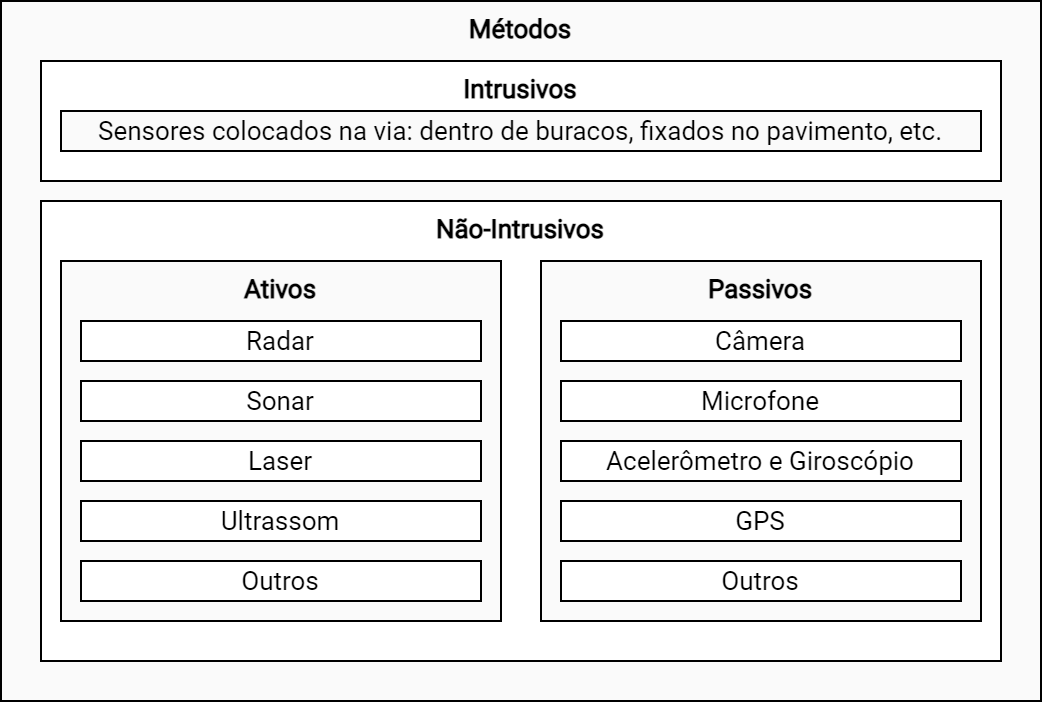
\includegraphics[width=0.9\linewidth]{figuras/fig_1.png}
  \fonte{Desenvolvido pelo autor.}
\end{figure}

Na abordagem não-intrusiva, são empregadas técnicas de sensoriamento passivo e ativo. As técnicas ativas requerem interação com o ambiente para produzir seus dados brutos, com a emissão de ondas no ambiente externo através de laser, ultrassom, sonar ou radar. As técnicas passivas, por sua vez, amostram seus dados sem necessitar interagir com o ambiente externo, como dados físicos ou imagens. Em comparação ao sensoriamento ativo, a abordagem passiva é considerada mais segura, não poluente e geralmente de menor custo. Essas características tornam estas técnicas mais interessantes para uso em larga escala, tal como sua aplicação em sistemas tipo do ADAS ou veículos autônomos. Dentre as soluções de sensoriamento passivo, a utilização de câmeras tem sido amplamente explorada nos últimos anos, com o desenvolvimento de soluções robustas em visão computacional. Contudo, o mesmo não ocorre com os sensores inerciais, representados por acelerômetro e giroscópio, os quais constituem uma alternativa importante a ser melhor explorada \cite{menegazzo2018,menegazzo2020}.

\section{Contextualização do Problema}

Classificados como não-intrusivos e passivos, os sensores inerciais se baseiam no princípio da inércia para produção de seus dados \cite{Braga2017}. Representados por giroscópios e acelerômetros, estes dispositivos produzem, respectivamente, sinais unidimensionais referentes a taxa de rotação e a força de aceleração em seus três eixos físicos \cite{Groves2013}. Neste estudo, estes sinais são resultantes da tração do veículo e das interações com o ambiente no qual ele trafega. Através da aplicação em veículos, sejam fixados diretamente na estrutura veicular ou embarcados em dispositivos móveis como \textit{smartphones} e \textit{tablets}, os sensores inerciais permitem a produção de uma grande diversidade de informações situacionais, conforme ilustra a \autoref{fig:percepcoes_veiculares}.

\begin{figure}[h]
  \centering
  \caption{Percepções veiculares produzidas através de dados de sensores inerciais}
  \label{fig:percepcoes_veiculares}
  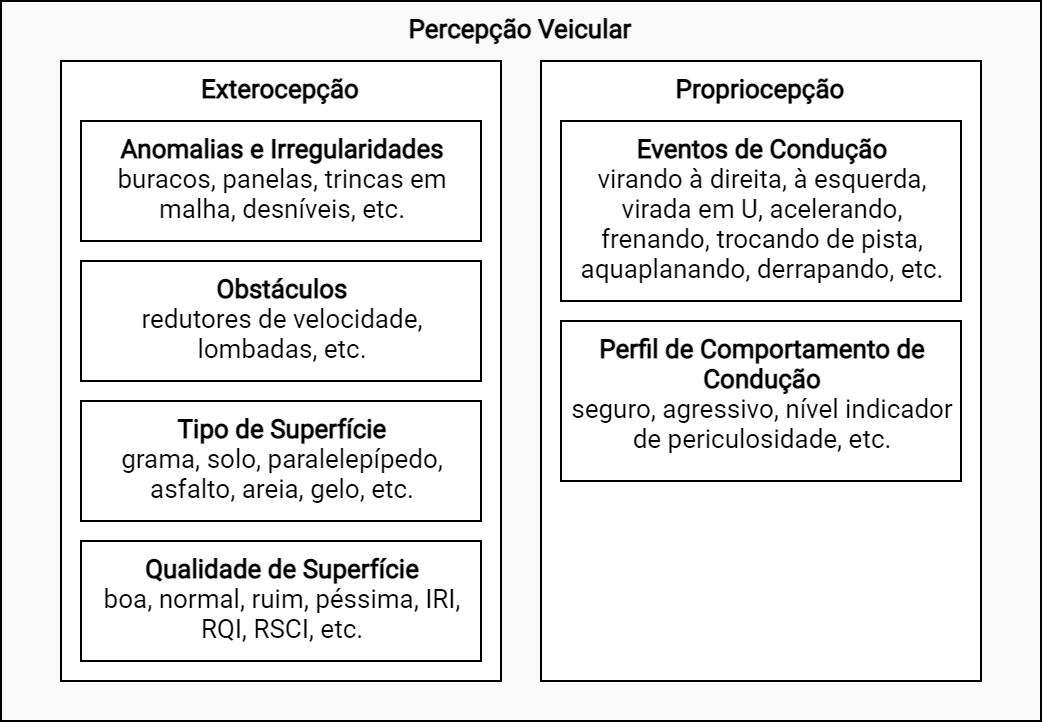
\includegraphics[width=0.9\linewidth]{figuras/fig_2.png}
  \fonte{Desenvolvido pelo autor.}
\end{figure}

Embora sejam diversas e relevantes as percepções veiculares produzidas, a utilização de sensores inerciais em ITS pouco avançou nos últimos anos. Através da Revisão Sistemática da Literatura (RSL) \cite{menegazzo2018,menegazzo2020}, foi observado que a maioria dos estudos da área apresenta foco na aplicação das percepções produzidas. Sendo assim, consistem em pesquisas na forma de prova de conceito, onde as soluções apresentadas para produção de percepções veiculares são simplistas e não aplicáveis a cenários do mundo real, devido a inadaptabilidade dos modelos. Contudo, entendemos que a adaptabilidade é um recurso essencial, onde a solução desenvolvida precisa apresentar um certo grau de confiabilidade quando aplicada em cenários não controlados onde há variações contextuais. Em uma análise comparativa, enquanto soluções baseadas em imagens/vídeos se mostram maduras, com análises em variações contextuais tais como avaliação em diferentes dimensões, marcações desbotadas, diferentes condições de iluminação e oclusão por causa de veículos ou pedestres \cite{Srimongkon2017, Patil2020}, o mesmo não ocorre com os modelos baseados em sinais de sensores inerciais. Nas aplicações desenvolvidas com estes sensores, os modelos analisam cenários controlados e limitados, sem considerar variações de condições no contexto que influenciam os sinais amostrados e, portanto, o resultado da solução final \cite{menegazzo2018,menegazzo2020}.

De acordo com \cite{Carlos2019}, nos últimos 10 anos se produziu uma literatura vasta sobre modelos para produzir informações situacionais a partir dos dados de sensores inerciais fixados no veículo ou embarcados nos \textit{smartphones}. Contudo, é necessário em novas pesquisas tornar os modelos mais inteligentes para traçar o perfil das estradas com detalhes reais \cite{Carlos2019}. Esta afirmação também é sustentada pelos resultados obtidos no levantamento do estado da arte \cite{menegazzo2018,menegazzo2020}, onde observa-se que para um modelo de percepção veicular operar de forma segura e confiável em cenários do mundo real, é necessário considerar os fatores de dependência que impactam nos sinais dos sensores inerciais. Estes fatores estão relacionados à diversidade contextual existente, onde o modelo pode ser aplicado a diferentes veículos, motoristas e ambientes. Considerar estes fatores no modelo o torna adaptável a diferentes condições, sendo este um requisito essencial para sua ampla utilização.

\section{Objetivos}

Nesta seção são detalhados o objetivo geral e específicos desta pesquisa.

\subsection{Objetivo Geral}

Este trabalho objetiva desenvolver modelos adaptativos para produção de percepções veiculares com emprego de sinais de sensores inerciais e técnicas de Inteligência Artificial (IA).  Para satisfazer o requisito de adaptabilidade, os modelos devem demonstrar boa capacidade de generalizar seu aprendizado quando submetido a contextos desconhecidos, os quais apresentam variações contextuais relacionadas as suas propriedades de dependência.

\subsection{Objetivos Específicos}

Os objetivos específicos deste trabalho são:

\begin{itemize}

\item Identificar o estado da arte acerca da produção de percepção veicular através de sinais de sensores inerciais;

\item Desenvolver uma infraestrutura e uma metodologia para coleta de dados brutos;

\item Produzir conjuntos de dados com variações contextuais das propriedades de dependência;

\item Desenvolver um modelo para classificação do tipo de superfície de pista, classificando os sinais dos sensores inerciais entre segmentos de terra, paralelepípedo ou asfalto;

\item Desenvolver um modelo para classificação da irregularidade de superfície de pista,  classificando os sinais dos sensores inerciais entre segmentos de qualidade ruim, regular ou boa;

\item Desenvolver um modelo para detecção de lombadas, através de sinais dos sensores inerciais;

\item Validar a adaptabilidade dos modelos através de um \textit{design} experimental, onde cada modelo será avaliado quanto a sua capacidade de generalização de aprendizado para contextos desconhecidos;

\end{itemize}

\section{Justificativa}

Para disseminar a utilização de ITS em suas mais variadas formas, mostra-se necessário tornar estes sistemas cada vez mais inteligentes. Para isto, é necessário dispor de mais fontes de dados, que estes dados sejam confiáveis, e que os dispositivos que os produzem não sejam prejudiciais à saúde humana quando aplicados em massa. Sendo assim, os sensores inerciais constituem uma fonte de dados alternativa, com grande potencial de melhorar as aplicações em ITS. Devido a sua abordagem passiva, se mostra um meio seguro, não poluente e de baixo custo. A segurança de sua aplicação em massa já foi amplamente validada, uma vez que todo \textit{smartphone} e \textit{tablet} possui um conjunto destes dispositivos. Os sinais produzidos pelos sensores permitem a produção de uma grande variedade de percepções veiculares, dentre exterocepções e propriocepções. Contudo, os atuais modelos de percepção veiculares baseados em sensores inerciais não são confiáveis, se mostrando o principal entrave para sua maior adoção.

A não confiabilidade nos modelos atuais se deve essencialmente a falta de adaptabilidade das soluções. Desta forma, os modelos desenvolvidos não mantêm sua efetividade quando aplicados em cenários diferentes do qual foi experimentado. Sendo assim, os estudos no estado da arte não consideram as variações contextuais pelas quais o modelo será submetido, e os fatores de dependência relacionados. Desta forma, o desenvolvimento de um modelo adaptativo de percepção se mostra de grande contribuição, seja aplicada na tomada de decisão humana ou artificial. Constituindo um aplicação meio para outros sistemas, diversas áreas dos ITS podem se beneficiar, como veículos autônomos, Sistemas Avançados de Controle de Veículos (\textit{Advanced Vehicle Control Systems} - AVCS), Sistemas Avançados de Informação ao Viajante (\textit{Advanced Traveler Information Systems} - ATIS), Sistemas Avançados de Gerenciamento de Tráfego (\textit{Advanced Traffic Management Systems} - ATMS), Sistemas Avançados de Gerenciamento de Transporte Público (\textit{Advanced Public Transport Management Systems} - APTMS), ADAS, entre outros \cite{Zhang2011,Singh2015}.

\subsection{Cenários de Aplicação}

Nesta seção são detalhados alguns cenários de aplicação dos modelos propostos.

\begin{description}

\item [Veículos Autônomo:] Um veículo equipado com sensores inerciais e auxiliares de suporte trafega em uma via. A irregularidade longitudinal da pista, correspondente ao conjunto dos desvios da superfície, é processada em relação a um plano de referência. Nesta análise, é estabelecido um índice de qualidade de conservação e identificado o tipo de pavimentação da via. Também são reconhecidos e classificados eventos transientes de percepção de ambiente, como obstáculos na via (lombadas, redutores de velocidade etc.), deficiências da superfície (buracos, solavancos etc.); e de propriocepção, como eventos de condução (virando à direita suave ou bruscamente, virando à esquerda, acelerando, frenando etc.). Disponibilizando estas informações através de uma interface ao agente inteligente que controla o veículo, o índice de qualidade de superfície e o tipo de pavimentação aferido são empregados no controle de velocidade veicular, sendo menor em vias mais irregulares e vice-versa. Esta decisão pode ser monitorada através dos eventos de condução e, se necessário, efetuado ajustes de comando. Os eventos transientes detectados de percepção de ambiente, utilizados na forma de evidências, auxiliam na convalidação de dados obtidos de sensores multimodais, tal qual por intermédio de visão computacional, corroborando hipóteses sobre o contexto no qual está inserido.

\item [Sistema Avançado de Assistência ao Motorista:] Em um sistema de \textit{vehicular crowdsensing} com sensoriamento oportunista, um \textit{crowdsourcer} utiliza um aplicativo de ADAS em seu computador de bordo ou \textit{smartphone}. Com os sensores inerciais anexados ao veículo ou embarcados nos dispositivos móveis, o aplicativo analisa as vibrações recebidas, para estabelecer conceitos qualitativos sobre a irregularidade de superfície e reconhecer eventos transientes, na forma de obstáculos e anomalias. Um servidor central recebe dados de vários \textit{crowdsourcers}, onde aplica-se um aprendizado baseado em reforço. Empregando a confiabilidade inicialmente estabelecida e a quantidade de detecções em diferentes fontes, a aplicação central realiza ajustes periódicos dos valores de confiabilidade dos dados, de forma que falsos positivos tenham progressivamente sua confiabilidade reduzida a zero, assim como algum evento transiente que deixe de existir, especialmente em função das manutenções realizadas na via. Com esse processamento no servidor, os dados atualizados são baixados pelos \textit{crowdsourcers}, de forma que o aplicativo ADAS utiliza-os para auxiliar o motorista, alertando-o sobre a velocidade acima da segura para uma pista com aquela qualidade de superfície, obstáculos e deficiências durante o trajeto.

\item [Sistema de Monitoramento de Infraestrutura de Transporte Terrestre:] Um veículo e\-qui\-pa\-do com sensores inerciais e auxiliares de suporte trafega em uma via. A irregularidade longitudinal da pista, correspondente ao conjunto dos desvios da superfície, é processada em relação a um plano de referência. Nesta análise, é estabelecido um índice de qualidade de conservação e identificado o tipo de pavimentação da via. Também são reconhecidos e classificados eventos transientes de percepção de ambiente, como obstáculos na via (lombadas, redutores de velocidade etc.), deficiências da superfície (buracos, solavancos etc.). Estas informações situacionais são salvas em um servidor remoto, com as respectivas coordenadas geodésicas. Posteriormente, estes dados são utilizados para definir a manutenção das vias, quando e onde deve ocorrer. Estes dados podem integrar relatórios governamentais, tais como o Relatório Gerencial produzido pela Confederação Nacional do Transporte (CNT), de forma a auxiliar direcionamento de investimentos públicos no modal de transporte terrestre.

\end{description}

\section{Contribuições}

Este trabalho apresenta diversas contribuições de aspecto teórico e aplicado. Com a produção de uma ampla revisão sistemática da literatura, foi realizado o levantamento do estado da arte na aplicação de sensores inerciais para produção de percepções veiculares. Através da análise deste levantamento, foram mapeados todos os fatores de dependência existentes no contexto de ITS que influenciam os sinais amostrados através de sensores inerciais. Este mapeamento, até então inexistente, é importante para que se possa desenvolver modelos de percepção veicular mais robustos, com adaptabilidade ao contexto. Junto a estes fatores, foram produzidos mapeamentos de aspectos diversos, que compreendem desde a etapa da coleta de dados, pré-processamento e processamento.

Com o estabelecimento do estado da arte e mapeamento de aspectos importantes nesta área de pesquisa, foi desenvolvida uma metodologia de coleta de dados, a qual compreende desde a criação da rede de sensores, referenciais de coleta e análise, colocação e posicionamento dos sensores na infraestrutura veicular, etc. Através dessa metodologia, foram produzidos nove conjuntos de dados com variações contextuais relacionadas aos fatores de dependência: diferentes veículos, motoristas e ambientes. Baseando-se nos conjuntos de dados, produzimos um \textit{design} experimental compreendendo as etapas de treinamento e validação dos modelos, de forma a ser possível avaliar a eficiência da generalização de aprendizado do modelo quando aplicado a um contexto desconhecido. Por fim, através de técnicas de \textit{Deep Learning} foram desenvolvidos três modelos adaptativos de percepção veicular, de forma que suas camadas de processamento fossem capazes de compreender as relações entre os dados e seus fatores de dependência. O primeiro modelo classifica o tipo de superfície de pista. O segundo, a qualidade da superfície. Por fim, o terceiro identifica lombadas na via.

Este projeto é inteiramente \textit{open-source}, disponibilizado no Github \footnote{https://github.com/Intelligent-Vehicle-Perception/Intelligent-Vehicle-Perception-Based-on-Inertial-Sensing-and-Artificial-Intelligence} \footnote{https://codigos.ufsc.br/lapix/intelligent-vehicle-perception-based-on-inertial-sensing}. Desta forma, os códigos-fonte utilizados na coleta de dados, para manipulação de sensores, amostragem e armazenamento dos sinais; no pré-processamento, com ajustes, combinação de dados, normalização, etc.; no processamento, com a classificação dos padrões; assim como os próprios datasets e modelos desenvolvidos, estão documentados e disponíveis publicamente, permitindo pesquisas futuras executarem, compararem e auditarem os experimentos. Convém mencionar que os conjuntos de dados produzidos são provavelmente os primeiros do tipo a serem disponibilizados publicamente, com coleta em múltiplos pontos e emprego de diversos sensores de abordagem passiva. Adicionalmente, o projeto conta com diversos materiais de divulgação científica, como vídeos dos sinais e modelos operando, e \textit{Jupyter Notebooks} com fundamentação teórica junto do código-fonte dos melhores modelos. Desta forma, estes materiais auxiliam na popularização deste tipo de sensoriamento em ITS, especialmente por atenuar a curva de aprendizado de novos pesquisadores na área.
 
\section{Estrutura do Trabalho}

Esta dissertação está estruturada em onze capítulos. No \autoref{cap:introducao}, é introduzido o problema de pesquisa, contextualização, justificativa, objetivos, contribuições sociais e científicas para a computação. No \autoref{cap:metodologia} é apresentada a metodologia utilizada neste trabalho, dentre os métodos para levantamento do estado da arte, coleta de dados, desenvolvimento e validação dos modelos. No \autoref{cap:fundamentacao} é discorrida a fundamentação teórica necessária para compreensão desta pesquisa. No \autoref{cap:revisao} é detalhada a revisão da literatura produzida e resultados obtidos, especificando as lacunas de pesquisa existentes com enfoque nas três percepções trabalhadas. No \autoref{cap:conjuntos_de_dados} é detalhada a metodologia de coleta de dados, rede de sensores produzida, referenciais adotados, colocação, posicionamento e configuração, além dos nove conjuntos produzidos. Nos Capítulos \ref{cap:classificacao_tipo_superficie_1} a \ref{cap:deteccao_lombadas} é apresentado a metodologia de desenvolvimento e validação, e os resultados obtidos do modelo adaptativo para classificação de superfície, classificação de qualidade e detecção de lombadas, respectivamente. Por fim, no \autoref{cap:materiais_resultantes} são apresentados os materiais resultantes e no \autoref{cap:conclusoes_discussoes} estão as considerações finais e sugestões de trabalhos futuros.

\chapter{Fundamentação Teórica}
\label{cap:fundamentacao}

Nesta seção são detalhados conceitos acerca dos materiais e métodos utilizados na pesquisa. Inicialmente é discorrido sobre o sensoriamento empregado, tipos de sensores, valores aferidos, entre outras características. Posteriormente, é apresentado o modelo matemático \textit{Quarter-Car} (QC), o qual descreve as mecânicas veiculares envolvidas no processo, e sua representação através das variáveis \textit{Golden Car Parameters}. Por fim, é detalhado o modelo computacional de \textit{Deep Learning} a ser utilizado, com o intuito de reconhecer e classificar os padrões de percepção veicular.

\section{Sensoriamento}

Nesta seção, são apresentados os sensores inerciais, os quais constituem fonte principal de dados do estudo. Em seguida, é discorrido sobre o sensor magnetômetro e GPS, uma vez que servem como sensores auxiliares, comumente utilizados em conjunto com os inerciais para prover informações adicionais. 

\subsection{Sensores Inerciais}

Os sensores inerciais constituem dispositivos que produzem sinais através do princípio da inércia \cite{Braga2017}. Estes sensores compreendem acelerômetros e giroscópios, de um ou mais eixos \cite{Beeby2004}. O acelerômetro mede a força de aceleração (em $m/s^2$ ou g = 9.8 $m/s^2$), enquanto que o giroscópio afere a taxa de rotação (em graus/segundo ou radianos/segundo), ambos sem a necessidade de um referencial externo \cite{Groves2013}. Sendo assim, a partir de um quadro de referência ou posição inicial destes sensores, forças externas que atuam sobre eles causam acelerações e mudanças de orientação (rotação) em um ou mais de seus eixos \cite{Kempe2011}. Neste estudo, essas forças são constituídas pela tração do veículo e pelas interações com o ambiente no qual ele trafega.

\subsubsection{Referenciais}

Os sensores inerciais não requerem nenhum referencial externo. Sendo assim, possuem seu próprio referencial, onde o sistema de coordenadas no qual os dados são amostrados é definido em relação a si próprios. No entanto, a análise dos dados com o objetivo de produzir percepção veicular deve ser realizada no referencial do veículo, como mostra a Figura \ref{fig:quadros_referencia}. Para isso, é necessário reorientar os eixos, mapeando os dados brutos de um sistema para outro.

\begin{figure}[h!]
  \centering
  \caption{Referenciais: (a) Referencial do sensor. (b) Referencial do sensor interno a dispositivos móveis. (c) Referencial da Terra. (d) Referencial do veículo.}
   \label{fig:quadros_referencia}
   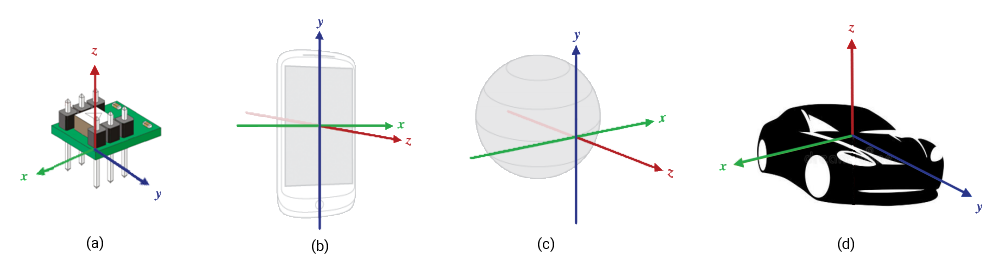
\includegraphics[width=1\textwidth]{figuras/fig2.png}
   \fonte{O autor.}
\end{figure}

A orientação dos dados é importante no processo de análise para que se possa utilizar os valores de acordo com o tipo de percepção a ser realizada. Sendo assim, baseando-se no referencial do veículo, os padrões de percepção de ambiente são mais evidentes na aceleração do eixo Z e na taxa de rotação do eixo Y. Já quanto aos padrões de propriocepção, mostram-se mais evidentes nos dados de aceleração nos eixos X e Y e nas taxas de rotação dos eixos X e Z. Para uma padronização de nomenclatura neste trabalho, serão usados os termos definidos nas Tabelas \ref{table:accelerometer_reference_frames} e \ref{table:gyroscope_reference_frames} para se referir aos dados em relação a cada um dos referenciais.

\begin{table}[h!]
    \caption{Referenciais para os dados de aceleração.}
    \label{table:accelerometer_reference_frames}
    \centering
    \begin{tabular}{clll}
        \toprule
        \textbf{Axis} & \textbf{Sensor} & \textbf{Veículo} & \textbf{Mundo} \\
        \toprule
        X & Aceleração em X & Aceleração Lateral & Aceleração Leste \\
        \midrule
        Y & Aceleração em Y & Aceleração Longitudinal & Aceleração Norte \\
        \midrule
        Z & Aceleração em Z & Aceleração Vertical & Aceleração Vertical (Mundo) \\
        \bottomrule
    \end{tabular}
    \fonte{O autor.}
\end{table}

\begin{table}[h!]
    \caption{Referenciais para os dados de taxa de rotação.}
    \label{table:gyroscope_reference_frames}
    \centering
    \begin{tabular}{clll}
        \toprule
        \textbf{Axis} & \textbf{Sensor} & \textbf{Veículo} & \textbf{Mundo} \\
        \toprule
        X & Taxa de Rotação Pitch & Taxa de Rotação Lateral & N/A \\
        \midrule
        Y & Taxa de Rotação Roll & Taxa de Rotação Longitudinal & N/A \\
        \midrule
        Z & Taxa de Rotação Yaw & Taxa de Rotação Vertical & N/A \\
        \bottomrule
    \end{tabular}
    \fonte{O autor.}
\end{table}

Para a reorientação dos eixos, duas estratégias foram identificadas nos estudos revisados: o posicionamento controlado e o mapeamento através de fórmulas baseadas nos ângulos de Euler. O posicionamento controlado consiste em uma técnica simples, onde sensor é colocado no veículo de forma que os eixos nos referenciais coincidam, ou seja, os eixos do sensor ficam alinhados com os eixos do veículo. Portanto, não é necessário aplicar pré-processamento para reorientação. Essa técnica é usada tanto para os dados do acelerômetro e do giroscópio. 

Os ângulos de Euler, por sua vez, aplicados apenas aos dados de aceleração, fornecem um meio de representar a orientação espacial tridimensional de qualquer referencial como uma composição de três rotações elementares. A orientação de referência pode ser tomada como uma orientação inicial a partir da qual o sistema de coordenadas gira para alcançar sua orientação real \cite{Singh2017}. Assim, essas fórmulas reorientam os dados brutos usando os ângulos fornecidos. Estes dois métodos são detalhados e analisados comparados no Capítulo \ref{cap:revisao}, em conjunto com as demais análises da literatura. 

\subsubsection{Fatores de Dependência}

Os valores amostrados através dos sensores inerciais, embora não dependam de um referencial externo para sua produção, são afetados por propriedades externas e internas aos sensores. Essas propriedades constituem fatores de dependência, que influenciam diretamente a amplitude e dispersão dos valores medidos. Através da tanto da análise da literatura, quando de experimentos exploratórios conduzidos, foi possível observar a existência de fatores de dependência classificados na forma de quatro propriedades, discutidas a abaixo. Para que uma solução desenvolvida possa ser adaptativa na forma que está sendo proposta, é necessário que o modelo considere todas estas propriedades no seu desenvolvimento.

\begin{description}
	
	\item [Propriedades Sensoriais:] 
	
	Quatro fatores de dependência estão relacionados às configurações e características dos sensores, sendo eles a orientação \cite{Kumar2017}, resolução, faixa de medição e taxa de amostragem. A orientação do sensor, conforme discutido na seção anterior, afeta a amostragem de dados no sistema de coordenadas correto. Portanto, o sensor deve ser colocado de forma a ficar alinhado com o sistema de coordenadas do veículo ou ter uma reorientação de eixos para esse referencial. Isso implica na confiabilidade dos dados existentes em cada eixo de análise, pois cada um deles visa atingir certa percepção veicular.

	O segundo e o terceiro fator estão fortemente correlacionados. A resolução é definida de acordo com a faixa de medição escolhida para o sensor. Portanto, é necessário que o sensor tenha uma faixa de medição adequada para poder amostrar os dados sem saturar, ou seja, que a faixa de medição do sensor não seja menor que os valores possíveis a serem monitorados. A resolução, estabelecida a partir da faixa de valores a serem analisados, fornece o quão próximo o valor medido é comparado ao valor real, no processo de quantização. Assim, devido à limitação do número de bits representado pelos sensores, quanto maior a faixa de medição, menor a resolução.
	
	Por fim, a taxa de amostragem descreve a frequência da amostragem de dados por segundo. A escolha desse valor deve levar em consideração não apenas o custo computacional de armazenamento e processamento dos dados amostrados, mas também se, a uma determinada velocidade, será possível obter amostras suficientes para realizar as percepções. Dessa forma, quando o veículo está em alta velocidade, percepções transientes, como buracos, precisam de uma taxa de amostragem satisfatória, para que seja possível adquirir alguma amostra desse evento.
	
	\item [Propriedades Veiculares:] em relação às mecânicas veiculares, o principal fator de dependência é o sistema de suspensão veicular \cite{Kumar2017, Wickramarathne2018}. O sistema de suspensão do veículo, com o objetivo de amortecer os impactos causados pela superfície da pista, faz com que os valores absolutos sejam reduzidos quando medidos acima da suspensão, como ocorre quando os sensores são embarcados em dispositivos móveis. Portanto, os valores amostrados nos sensores anexados no veículo abaixo da suspensão não apresentam essa interferência, embora ainda recebam um pequeno amortecimento causado pelo pneu. Sendo assim, para realizar as percepções em diferentes veículos, deve-se considerar que cada um possui um sistema de suspensão diferente, sendo mais ou menos eficiente.

	\item [Propriedades Ambientais:] estas propriedades não abordadas em trabalhos relacionados, não são tão evidentes, embora necessitem ser consideradas na modelagem da adaptação. Seus fatores de dependência se relacionam com questões climáticas, como superfície de pista com água ou de pouco atrito, que levam a aquaplanagem e derrapagem. Sendo assim, são percepções que implicam na percepção de outras, ou seja, percepções que dependem de percepções. O mesmo ocorre com a variabilidade de superfície, onde a identificação de eventos transientes como buracos e lombadas dependem diretamente do tipo de pavimento que existe na pista, e se existe. Da mesma forma, o dinamismo do estado de conservação de um tipo de pavimento deve ser considerado para detectá-lo corretamente.

	\item [Propriedades de Condução:] as propriedades de condução, intrinsecamente relacionadas as propriedades veiculares, dizem respeito as ações de quem controla o veículo. Nesse sentido, o principal fator de dependência a ser considerado é a velocidade longitudinal \cite{Brunauer2016, Douangphachanh2013, Gueta2017, Kumar2017, Lima2016, M.2017, Nalavde2015, Singh2017}. A velocidade do veículo possui duas implicações. Uma vez que as curvas são feitas em todos os eixos do sistema de coordenadas do veículo, ocorre a produção do componente de força centrífuga. Portanto, as acelerações medidas dependem diretamente da velocidade aplicada. A segunda implicação da velocidade está na distribuição no tempo dos valores amostrados. Em velocidades mais baixas, mais amostras do evento são coletadas e, com o veículo em velocidades diferentes, diferentes quantidades de amostras são obtidas.

\end{description}

\subsection{Magnetômetro}

O magnetômetro é um sensor auxiliar comumente embarcado com os sensores inerciais devido sua função. Este sensor mede o campo geomagnético ambiental (em $\mu$T) em seus três eixos físicos \cite{Sattar2018}. Sendo assim, é geralmente aplicado junto aos ângulos de Euler para dar orientação aos dados e empregado com os dados de aceleração para aproximar dados de localização e velocidade mais rapidamente, uma vez que a taxa de amostragem do GPS é pequena.

\subsection{GPS}

O Sistema de Posicionamento Global (\textit{Global Positioning System} - GPS) consiste de um sistema de satélites que orbitam o planeta, auxiliando receptores em terra a determinar sua localização \cite{Milette2012}. Sendo assim, além dos dados geodésicos de latitude e longitude, o receptor GPS também afere sua velocidade. Embora preciso, este sistema possui uma taxa de amostragem baixa em relação aos demais sensores, cerca de 1Hz.

\section{Quarter Car}

O modelo matemático \textit{Quarter Car} (QC) descreve as variáveis da dinâmica veicular, conforme ilustra a Figura \ref{fig:quarter_car}. O modelo QC possui propriedades relacionadas a roda, suspensão e amortecimento. A propriedade de massa suspensa do veículo (Ms), fica acima da suspensão e representa um quarto da massa veicular. A propriedade de massa não suspensa (Mu), abaixo da suspensão, inclui a massa de uma roda e do sistema de suspensão conectado a ela. Entre as massas, existe a suspensão feita da mola (Ks) e de um amortecedor (C), que suporta a massa suspensa. Uma vez que a massa não suspensa está em contato direto com a superfície da pista, existe a rigidez do pneu (Kt) e a capacidade de absorção do pneu (Ct) impactando nos valores de força \cite{Yafeai2019}.

\begin{figure}[h!]
  \centering
  \caption{O modelo Quarter Car.}
   \label{fig:quarter_car}
   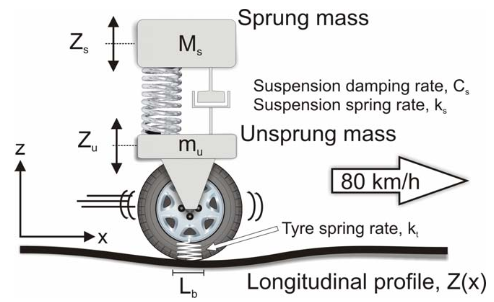
\includegraphics[width=0.6\textwidth]{figuras/fig2_2.png}
   \fonte{\cite{Loizos2008}}
\end{figure}

Através das diversas fórmulas que compõem o modelo, foram criados valores padrões para estas propriedades, denominados \textit{Golden Car Parameters} \cite{Loizos2008}, conforme detalha a Tabela \ref{table:golden_car_parameters}.

\begin{table}[h!]
    \caption{Os parâmetros Golden Car.}
    \label{table:golden_car_parameters}
    \centering
    \begin{tabular}{clll}
        \toprule
        \textbf{Parâmetro} & \textbf{Valor} \\
        \toprule
        Ks/Ms & 63,3 \\
        \midrule
        Kt/Ms & 653 \\
        \midrule
        Cs/Ms & 6 \\
        \midrule
        Mu/Ms & 0,15 \\
        \bottomrule
    \end{tabular}
    \fonte{\cite{Loizos2008}}
\end{table}

\section{Deep Learning}

Com o desenvolvimento do aprendizado de máquina, especialmente a partir de 2006, surgiu nesta área um segmento denominado aprendizado profundo (\textit{Deep Learning}) \cite{Deng2014}. Até então, a extração características importantes que bem representassem os dados parametrizados à uma técnica de reconhecimento de padrões, constituía um problema central. Sendo assim, as técnicas existentes apresentavam a grande dificuldade de se extrair, em um pré-processamento, características de alto nível através de dados brutos \cite{Goodfellow2016}. 

Com o desenvolvimento do \textit{Deep Learning}, esse problema foi solucionado, sendo introduzidas representações que são expressadas em termos de outras, construindo conceitos complexos através de conceitos simples \cite{Goodfellow2016}. Nessa abordagem, tornou-se possível construir modelos computacionais compostos de múltiplas camadas de processamento para aprender a representação dos dados com diversos níveis de abstração \cite{LeCun2015}. Sendo assim, o aprendizado profundo descobre uma estrutura complexa em grandes conjuntos de dados usando o algoritmo de retropropagação para calcular como alterar seus parâmetros internos, os quais são usados para calcular a representação em cada camada a partir da representação na camada anterior \cite{LeCun2015}.

Com este novo paradigma, foram melhorados drasticamente o estado da arte em reconhecimento de fala, reconhecimento visual de objetos, detecção de objetos e muitos outros domínios \cite{LeCun2015}. Os diversos métodos presentes nessa categoria podem ser classificados entre redes profundas para aprendizado não supervisionado ou generativo, redes profundas para aprendizado supervisionado e redes profundas híbridas \cite{Deng2014}. Na categoria de redes profundas para aprendizado supervisionado existem as redes do tipo \textit{Long Short-Term Memory} (LSTM), utilizadas neste trabalho e discorridas na próxima seção.

\subsection{Long Short-Term Memory}

A \textit{Long Short-Term Memory} (LSTM) constitui um tipo de Rede Neural Recorrente (\textit{Recurrent Neural Network} - RNN) considerada ideal para predição e classificação de séries temporais, substituindo muitas abordagens tradicionais por \textit{Deep Learning} \cite{Zaccone2017}. Nesta abordagem, introduzindo o conceito de célula de memória e auto-loops conforme a Figura \ref{fig:cell_lstm}, a rede pode manter valores por um período curto ou longo, como uma função de suas entradas. Assim, a célula consegue se lembrar daquilo que é importante, e não apenas do último valor computado \cite{Jones2017}.

\begin{figure}[h!]
  \centering
  \caption{Célula de memória da LSTM com auto-loop.}
   \label{fig:cell_lstm}
   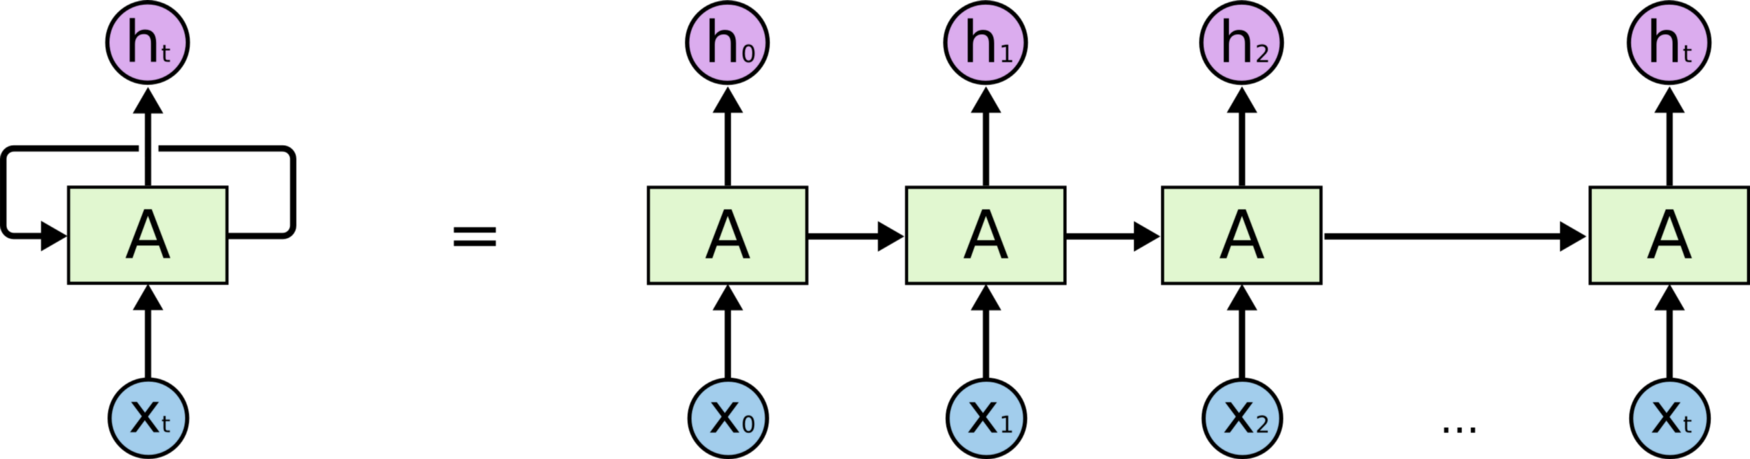
\includegraphics[width=1\textwidth]{figuras/fig2_3.png}
   \fonte{\cite{Junior2019}}
\end{figure}

Cada célula de memória de uma LSTM possuí três portas que controlam o fluxo de informações para dentro e fora da célula. Estas são a porta de entrada (\textit{input gate}), a porta de saída (\textit{output gate}) e a porta de esquecimento (\textit{forget gate}). As portas possuem pesos, onde os valores computados seguem um fluxo no qual resultam em alterações no estado de célula. Sendo assim, inicialmente tem-se a porta de esquecimento, responsável por decidir quais dados devem ser mantidos na memória e quais devem ser esquecidos \cite{Nguyen2018}. Isso permite que a célula se lembre de dados anteriores importantes, ou apenas de novos dados, esquecendo os anteriores. Em seguida, a porta de entrada é responsável por controlar quando novas informações podem entrar na memória. Finalmente, a porta de saída controla quais as informações contidas no próximo estado da célula.\cite{Jones2017}

\begin{figure}[h!]
  \centering
  \caption{Portas da célula de memória da LSTM.}
   \label{fig:cell_lstm_gates}
   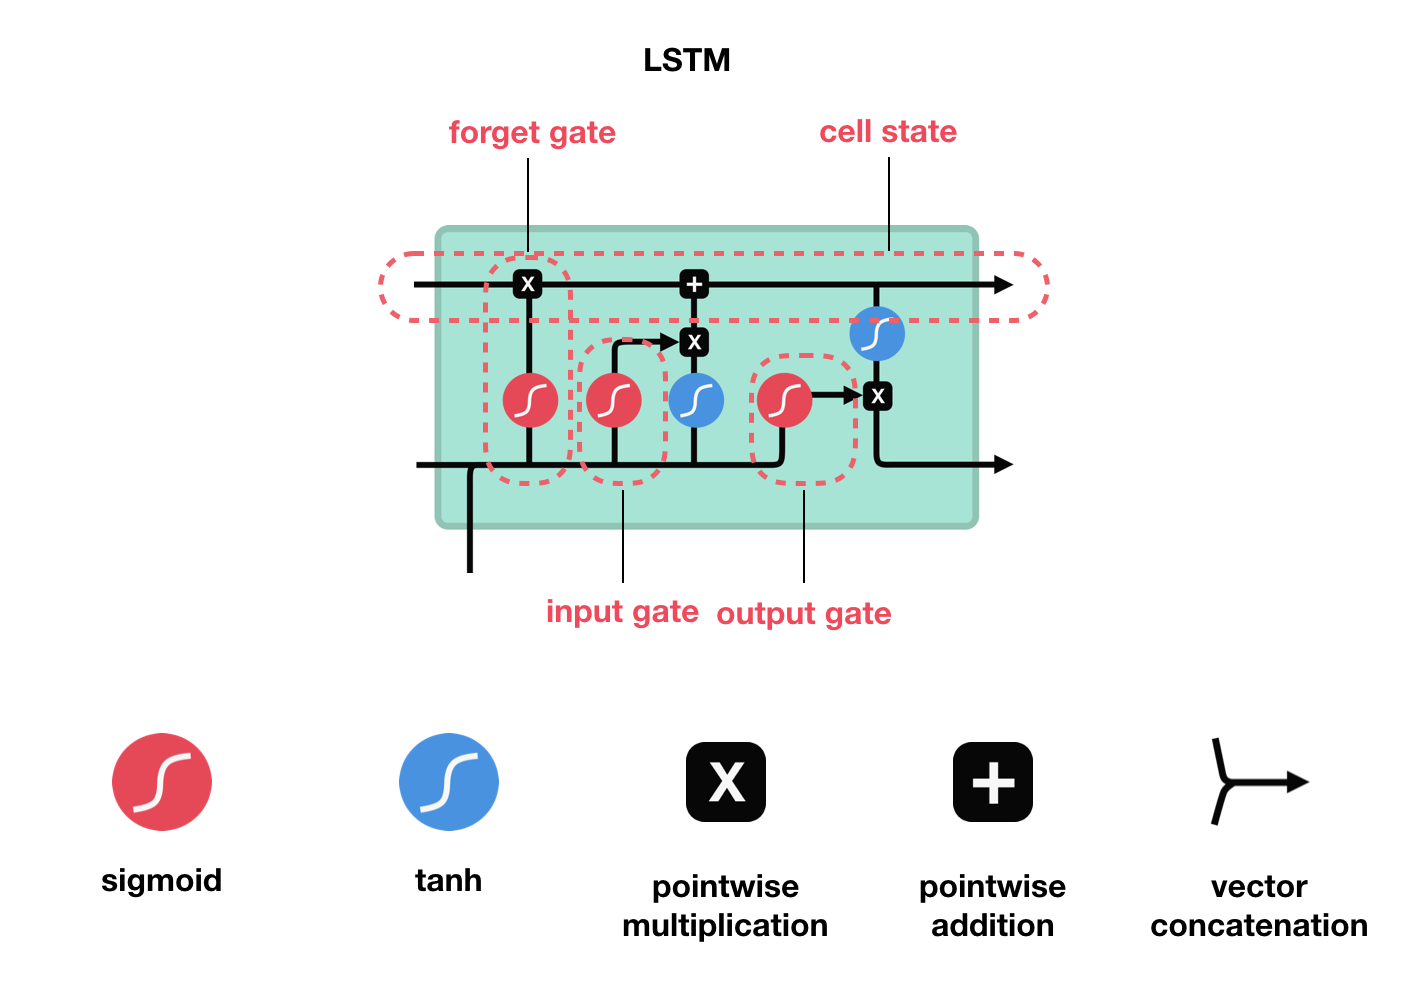
\includegraphics[width=1\textwidth]{figuras/fig2_3_1.png}
   \fonte{\cite{Nguyen2018}}
\end{figure}

\chapter{Fundamentação Teórica}
\label{cap:fundamentacao}

Nesta seção são detalhados conceitos acerca dos materiais e métodos utilizados na pesquisa. Inicialmente é discorrido sobre o sensoriamento empregado, tipos de sensores, valores aferidos, entre outras características. Posteriormente, é apresentado o modelo matemático \textit{Quarter-Car} (QC), o qual descreve as mecânicas veiculares envolvidas no sistema de suspensão. Em seguida, são detalhados as técnicas de IA utilizadas com o intuito de reconhecer e classificar os padrões de percepção veicular, dentre técnicas \textit{Machine Learning} clássico e \textit{Deep Learning}. Por fim, são apresentadas as métricas de avaliação adotadas.

\section{Sensoriamento}

Nesta seção, são apresentados os sensores inerciais, os quais constituem fonte principal de dados do estudo. Em seguida, é discorrido sobre o sensor magnetômetro e GPS, uma vez que servem como sensores auxiliares, comumente utilizados em conjunto com os inerciais para prover informações adicionais. 

\subsection{Sensores Inerciais}

Os sensores inerciais constituem dispositivos que produzem sinais através do princípio da inércia \cite{Braga2017}. Estes sensores compreendem acelerômetros e giroscópios, de um ou mais eixos \cite{Beeby2004}. O acelerômetro mede a força de aceleração (em $m/s^2$ ou g = 9.8 $m/s^2$), enquanto que o giroscópio afere a taxa de rotação (em graus/segundo ou radianos/segundo), ambos sem a necessidade de um referencial externo \cite{Groves2013}. Sendo assim, a partir de um quadro de referência ou posição inicial destes sensores, forças externas que atuam sobre eles causam acelerações e mudanças de orientação (rotação) em um ou mais de seus eixos \cite{Kempe2011}. Em síntese, são sensores que necessitam de movimento para produção de dados. Neste estudo, estes movimentos são resultantes das forças produzidas pela tração do veículo e pelas interações com o ambiente no qual ele trafega.

\subsection{Magnetômetro}

O magnetômetro é um sensor auxiliar comumente embarcado com os sensores inerciais em um mesmo módulo. Este sensor, também de abordagem passiva, mede o campo geomagnético ambiental (em $\mu$T) em seus três eixos físicos \cite{Sattar2018}. Sendo assim, é geralmente aplicado junto aos ângulos de Euler para dar orientação aos dados, reorientando para o referencial da terra. Também é empregado em conjunto com os dados de aceleração para estimar a localização e velocidade mais rapidamente, uma vez que a taxa de amostragem do GPS é muito mais lenta que a dos sensores inerciais.

\subsection{Global Position System}

O Sistema de Posicionamento Global (\textit{Global Positioning System} - GPS) consiste de um sistema de satélites que orbitam o planeta, auxiliando receptores em terra a determinar sua localização \cite{Milette2012}. Sendo assim, além dos dados geodésicos de latitude e longitude, o receptor GPS também afere a velocidade do objeto que contém o sensor. Embora preciso, este sistema possui uma taxa de amostragem baixa em relação aos demais sensores, cerca de 1Hz.

\section{Quarter Car}

O modelo matemático \textit{Quarter Car} (QC) descreve as variáveis da dinâmica veicular, conforme ilustra a \autoref{fig:quarter_car}. O modelo QC possui propriedades relacionadas a roda, suspensão e amortecimento. A propriedade de massa suspensa do veículo $m_s$, fica acima da suspensão e representa um quarto da massa veicular. A propriedade de massa não suspensa $m_u$, abaixo da suspensão, inclui a massa de uma roda e do sistema de suspensão conectado a ela. Entre as massas, existe uma suspensão feita de mola com uma taxa de suspensão $K_s$, e de um amortecedor com uma taxa de amortecimento $C_s$, os quais suportam a massa suspensa. Uma vez que a massa não suspensa está em contato direto com a superfície da pista, existe a rigidez do pneu e sua  capacidade de absorção representadas pela taxa de amortecimento do pneu $K_t$ \cite{Yafeai2019,Loizos2008}. Logo, uma força que parte da superfície da pista atingindo o pneu, será irradiada para todos estes componentes, onde será suavizada pelo deslocamento de massa suspensa $Z_s$ e da massa não suspensa $Z_u$, antes de chegar a parte superior do veículo.

\begin{figure}[h]
  \centering
  \caption{O modelo Quarter Car.}
   \label{fig:quarter_car}
   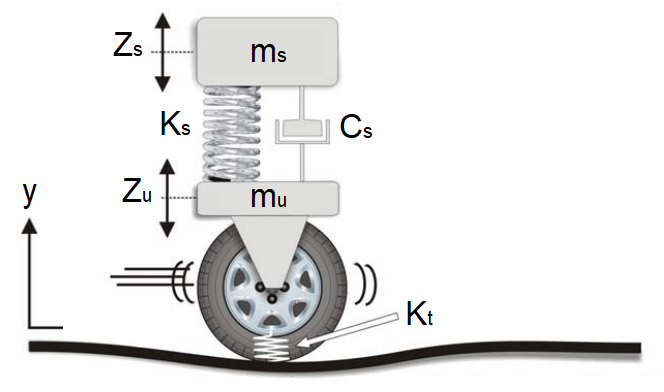
\includegraphics[width=0.8\textwidth]{figuras/fig_4.png}
   \fonte{Adaptado de \cite{Loizos2008}}
\end{figure}

Os valores das variáveis do modelo QC são definidos de acordo com cada veículo, dado as diferentes estruturas veiculares existentes. Este modelo conta com diversas fórmulas que descrevem o relacionamento entre todas as suas variáveis. Os parâmetros do modelo são essenciais na aplicação de metodologias internacionais para indexação da irregularidade, como o IRI, para estabelecer a qualidade da via. De forma a simplificar as fórmulas do QC, foram criados valores padrões para as propriedades, denominados \textit{Golden Car Parameters}. Estas propriedades, detalhadas na \autoref{table:golden_car_parameters}, foram estabelecidas considerando um cenário padrão, onde o veículo é dirigido a uma velocidade constante de 80 $km/h$ \cite{Loizos2008}.

\begin{table}[h]
    \caption{Os parâmetros \textit{Golden Car}}
    \label{table:golden_car_parameters}
    \centering
    \small
    \begin{tabular}{cl}
        \toprule
        \textbf{Parâmetro} & \textbf{Valor} \\
        \toprule
        $K_s/m_s$ & 63,3 \\
        \midrule
        $K_t/m_s$ & 653 \\
        \midrule
        $C_s/m_s$ & 6 \\
        \midrule
        $m_u/m_s$ & 0,15 \\
        \bottomrule
    \end{tabular}
    \fonte{Adaptado de \cite{Loizos2008}}
\end{table}

\section{Técnicas Clássicas de Machine Learning}

Com o desenvolvimento da Inteligência Artificial, diversas técnicas surgiram para resolver problemas de classificação, regressão e previsão. Dentre as técnicas clássicas de \textit{clustering} e aprendizado de máquina supervisionado, neste trabalho foram desenvolvidos modelos de \textit{K-Means Clustering} (KMC), \textit{K-Nearest Neighbors} (KNN) e \textit{Support Vector Machines} (SVM), detalhadas nas próximas subseções.

\subsection{K-Means Clustering}

O KMC consiste de uma técnica não supervisionada para agrupamento de dados (\textit{clustering}), que permite identificar agrupamentos (\textit{clusters}) de dados semelhantes, conforme ilustra a \autoref{fig:execucao_kcm}. Neste método, partindo de um conjunto de dados não rotulados (1), são criadas aleatoriamente centróides para cada um dos \textit{k clusters} (2). Em seguida, cada dado é atribuído a um dos \textit{clusters} baseando-se em uma métrica de distância, como a Euclidiana, em relação à centroide do \textit{cluster} (3, 4). Iterativamente, a centroide de cada \textit{clusters} é recalculada com base na média dos dados (5), e as distâncias novamente recalculadas (6, 7), até que as centróides sejam estabilizadas, ou o número máximo de iterações atingido \cite{foley2019,nisbet2009}.

\begin{figure}[h]
  \centering
  \caption{Execução da técnica KMC.}
   \label{fig:execucao_kcm}
   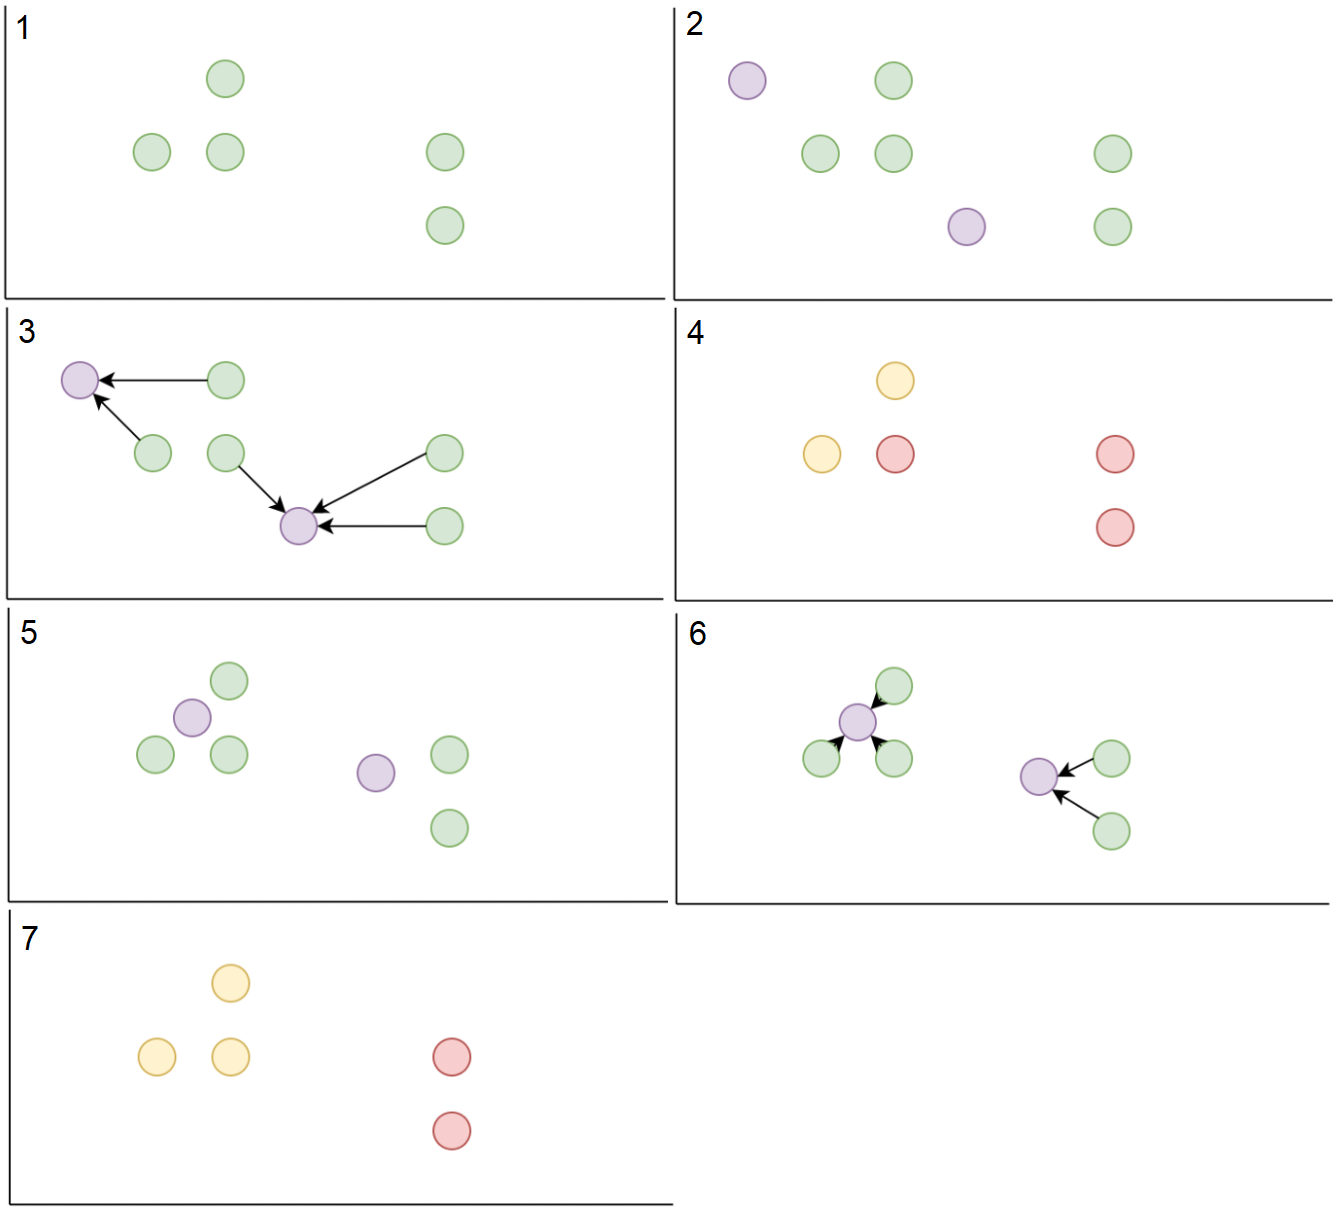
\includegraphics[width=0.7\textwidth]{figuras/fig_5.png}
   \fonte{Adaptado de \cite{i2020}}
\end{figure}

\subsection{K-Nearest Neighbors}

O KNN consiste de uma técnica para classificação a qual se baseia em métricas de similaridades entre os dados para reconhecer padrões. Desta forma, para um novo dado a ser classificado é calculada a distância entre ele e cada um dos dados de treinamento, identificando os k vizinhos mais próximos. A classe do novo dado é definida como aquela mais comum entre seus k vizinhos, conforme ilustra a \autoref{fig:execucao_knn} \cite{Khandelwal2018}.

\begin{figure}[h]
  \centering
  \caption{Execução da técnica KNN.}
   \label{fig:execucao_knn}
   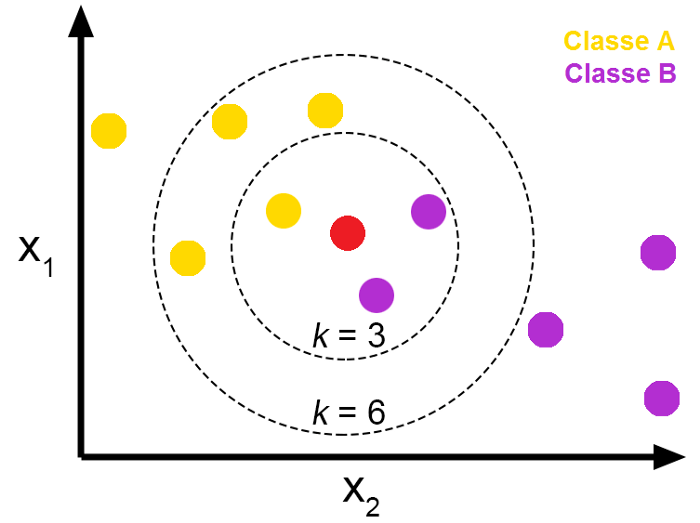
\includegraphics[width=0.4\textwidth]{figuras/fig_6.png}
   \fonte{\cite{Jose2018}}
\end{figure}

\subsection{Support Vector Machines}

O SVM é uma técnica de aprendizado supervisionado aplicada em classificação, onde se busca por um hiperplano ideal que separa as classes de dados, conforme ilustra a \autoref{fig:execucao_svm}. O algoritmo se inicia com a busca pelos pontos mais próximos ao hiperplano que separa as classes. Esses pontos são chamados de vetores de suporte. Na sequencia, é calculada a distância entre o hiperplano e estes vetores. Essa distância é chamada de margem, a qual o SVM busca maximizar, de forma a encontrar o hiperplano ideal \cite{Pupale2019}. Em problemas não lineares, como é o caso deste, é necessário a utilização do hiperparâmetro kernel, o qual converte problema não separável em problema separável, para que o SVM possa classificar \cite{Shubham2018}.

\begin{figure}[h]
  \centering
  \caption{Execução da técnica SVM.}
   \label{fig:execucao_svm}
   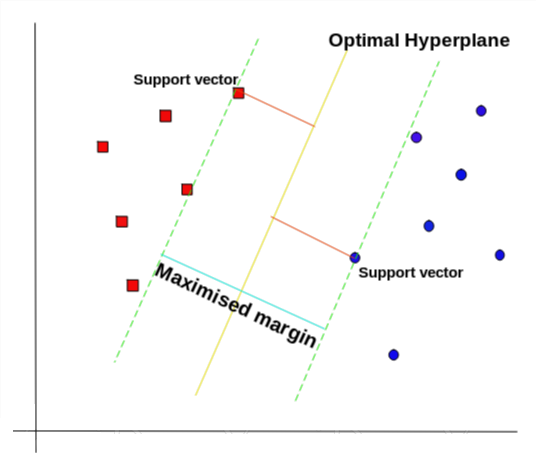
\includegraphics[width=0.7\textwidth]{figuras/fig_7.png}
   \fonte{\cite{Pupale2019}}
\end{figure}

\section{Técnicas de Deep Learning}

Com o desenvolvimento do aprendizado de máquina, especialmente a partir de 2006, surgiu nesta área um segmento denominado aprendizado profundo (\textit{Deep Learning}) \cite{Deng2014}. Até então, a extração características importantes que bem representassem os dados parametrizados à uma técnica de reconhecimento de padrões, constituía um problema central. Sendo assim, as técnicas existentes apresentavam a grande dificuldade de se extrair, em um pré-processamento, características de alto nível através de dados brutos \cite{Goodfellow2016}. 

Com o desenvolvimento do \textit{Deep Learning}, esse problema foi solucionado, sendo introduzidas representações que são expressadas em termos de outras representações, construindo conceitos complexos através de conceitos simples \cite{Goodfellow2016}. Nessa abordagem, tornou-se possível construir modelos computacionais compostos de múltiplas camadas de processamento para aprender a representação dos dados com diversos níveis de abstração \cite{LeCun2015}. Sendo assim, o aprendizado profundo descobre uma estrutura complexa em grandes conjuntos de dados utilizando do algoritmo de retropropagação para calcular como alterar seus parâmetros internos, os quais são usados para estabelecer a representação em cada camada a partir da representação obtida na camada anterior \cite{LeCun2015}.

Com este novo paradigma, foram melhorados drasticamente o estado da arte em reconhecimento de fala, reconhecimento visual de objetos, detecção de objetos e muitos outros domínios \cite{LeCun2015}. Os diversos métodos presentes nessa categoria podem ser classificados entre redes profundas para aprendizado não supervisionado ou generativo, redes profundas para aprendizado supervisionado e redes profundas híbridas \cite{Deng2014}. Neste trabalho, foram utilizadas redes  profundas para aprendizado supervisionado do tipo \textit{Long Short-Term Memory} (LSTM), \textit{Convolutional Long Short-Term Memory} (ConvLSTM), \textit{Gated Recurrent Unit} (GRU)  e \textit{Convolutional Neural Network} (CNN), assim como redes profundas híbridas do tipo \textit{Convolutional Neural Network Long Short-Term Memory} (CNN-LSTM), discorridas nas próximas seções.

\subsection{Long Short-Term Memory}

A LSTM constitui um tipo de Rede Neural Recorrente (\textit{Recurrent Neural Network} - RNN) considerada ideal para predição e classificação de séries temporais, substituindo muitas abordagens tradicionais por \textit{Deep Learning} \cite{Zaccone2017}. Suas aplicações envolvem previsão ou classificação de séries temporais \cite{Zaccone2017}, tais como previsão de velocidade de tráfego, modelagem de linguagem, reconhecimento de fala, aprendizagem de gramática, modelagem de áudio, reconhecimento de caligrafia, etc. \cite{Bianchi2017}. Nesta abordagem, introduzindo o conceito de estado de célula (memória) e \textit{auto-loops} conforme ilustra a \autoref{fig:cell_lstm}, a rede pode manter valores por um curto ou longo período de tempo, como uma função de suas entradas. Assim, a célula consegue se lembrar daquilo que é importante, e não apenas do último valor computado \cite{Jones2017}, de forma que informações relevantes de entradas anteriores são retidas e utilizadas para alterar a saída atual \cite{Zebin2018}.

\begin{figure}[h]
  \centering
  \caption{Célula de uma LSTM com \textit{auto-loop}.}
   \label{fig:cell_lstm}
   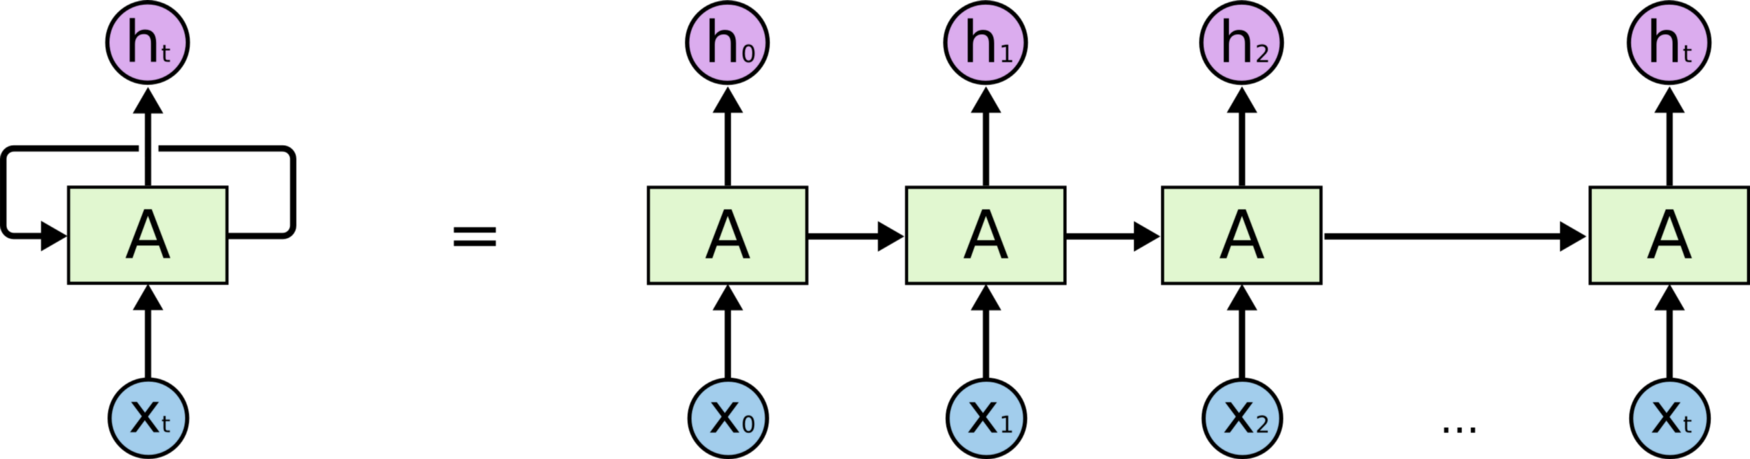
\includegraphics[width=0.8\textwidth]{figuras/fig_8.png}
   \fonte{\cite{Junior2019}}
\end{figure}

Cada célula de uma LSTM possuí três portas que controlam o fluxo de informações para dentro e fora da célula, ilustrado na \autoref{fig:cell_lstm_gates}. Estas são: a porta de entrada (\textit{input gate}), a porta de saída (\textit{output gate}) e a porta de esquecimento (\textit{forget gate}). As portas possuem pesos, onde os valores computados seguem um fluxo no qual resultam em alterações no estado de célula. Sendo assim, inicialmente tem-se a porta de esquecimento, responsável por decidir quais dados devem ser mantidos na memória e quais devem ser esquecidos \cite{Phi2020}. Isso permite que a célula se lembre de dados anteriores importantes, ou apenas de novos dados, esquecendo os anteriores. Em seguida, a porta de entrada é responsável por controlar quando novas informações podem entrar na memória. Finalmente, a porta de saída controla quais as informações contidas no próximo estado da célula \cite{Jones2017}.

\begin{figure}[h]
  \centering
  \caption{Componentes de uma célula de LSTM.}
   \label{fig:cell_lstm_gates}
   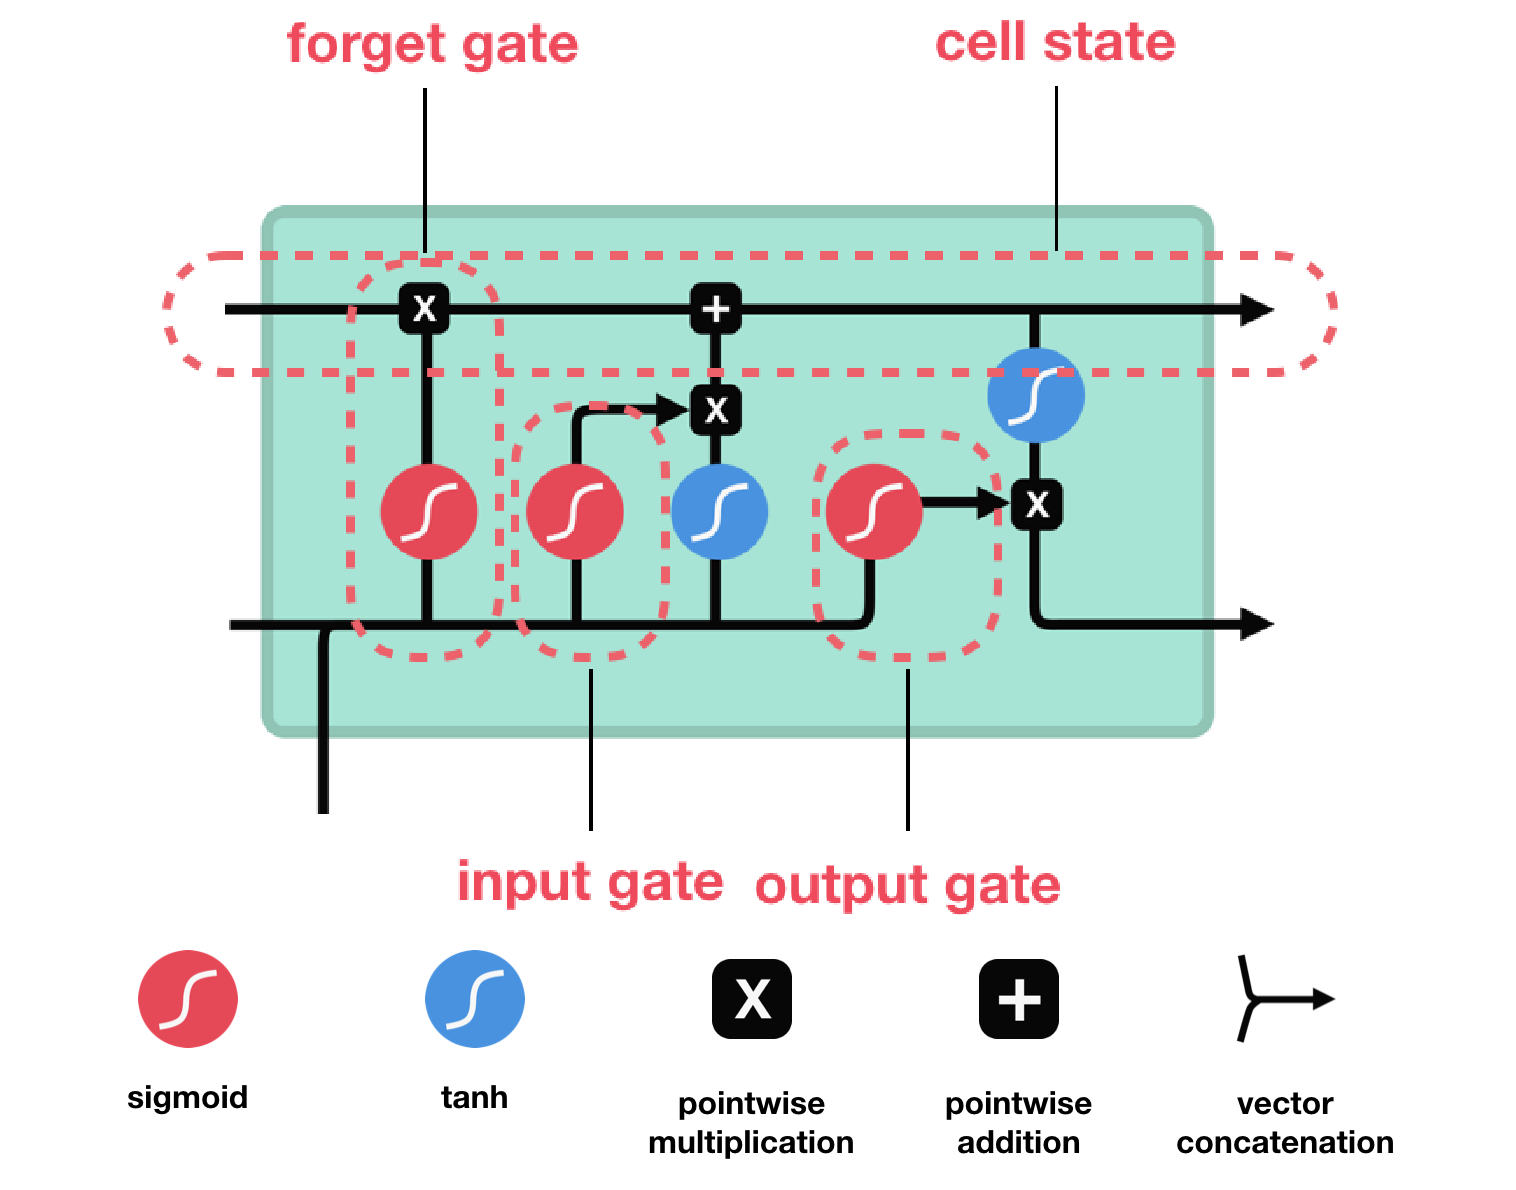
\includegraphics[width=0.8\textwidth]{figuras/fig_9.png}
   \fonte{Adaptado de \cite{Phi2020}}
\end{figure}

\subsection{Gated Recurrent Unit}

A GRU consiste de um tipo de RNN com o mesmo propósito da LSTM, embora considerada uma melhoria em relação a anterior, utilizando menos portas e parâmetros \cite{Kumar2019,Bianchi2017}. Em razão disso, redes GRU superaram a performance de redes LSTM em várias aplicações, treinando e convergindo mais rápido, se mostrando computacionalmente menos custosas e igualmente eficientes \cite{Kumar2019,Bianchi2017}. Empregada também em classificação e previsão de séries temporais, este tipo de rede ajuda na recuperação de informações em escalas de tempo distintas \cite{Bianchi2017,Kumar2019}. 

Cada célula de uma GRU possuí um estado de célula (memória) que utiliza de um estado escondido (\textit{hidden state}) para transferir a informação, com é feito na LSTM. Contudo, a GRU utiliza de apenas duas portas, conforme ilustra a \autoref{fig:cell_gru_gates}: a porta de reinicialização (\textit{reset gate}) e a porta de atualização (\textit{update gate}). A porta de atualização opera de forma similar às portas de esquecimento e a de entrada de uma LSTM, decidindo quais informações descartar e quais informações novas adicionar a memória. A porta de reinicialização, por sua vez, é utilizada para decidir quais informações do passado devem ser esquecidas \cite{Phi2020}.

\begin{figure}[h]
  \centering
  \caption{Componentes de uma célula de GRU.}
   \label{fig:cell_gru_gates}
   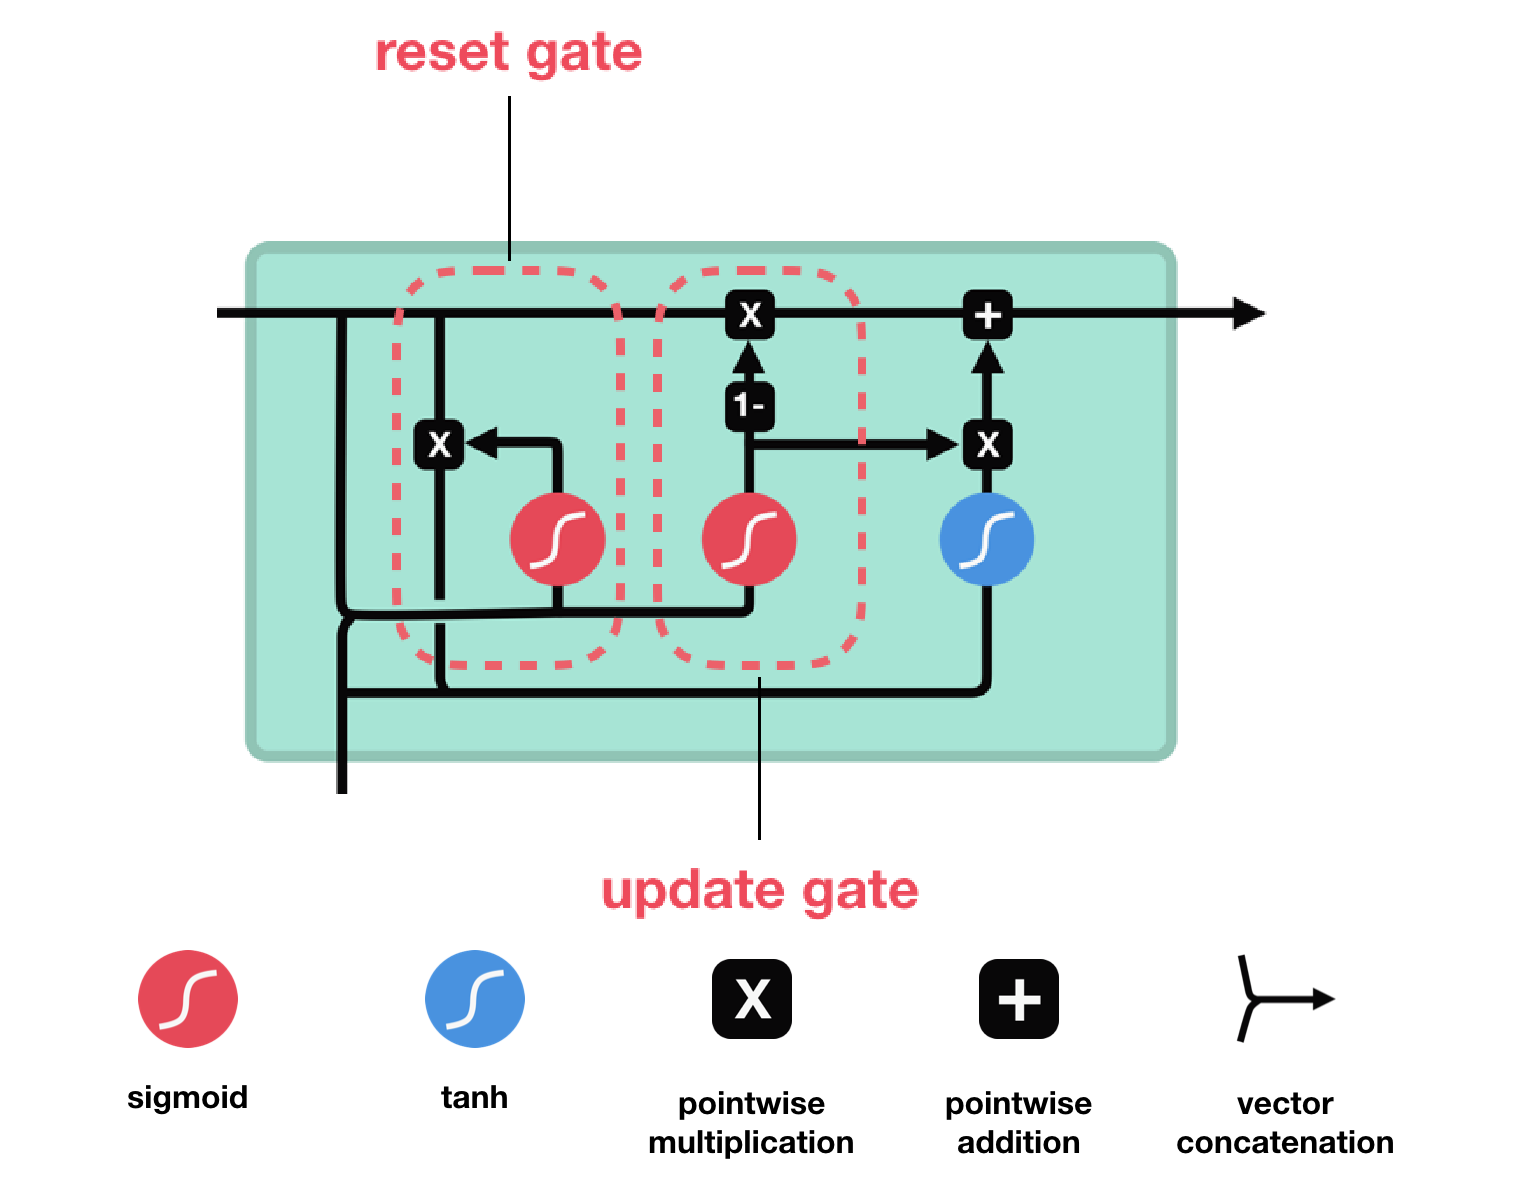
\includegraphics[width=0.8\textwidth]{figuras/fig_10.png}
   \fonte{Adaptado de  \cite{Phi2020}}
\end{figure}

\subsection{Convolutional Neural Network}

A CNN é um tipo de rede neural projetada para tratar eficientemente dados de imagem, se mostrando efetiva em aplicações de visão computacional, como classificação de imagem, localização de objetos, etc. \cite{Brownlee2018}. Através da aplicação de convoluções, este tipo de rede é capaz de aprender como extrair características de alto nível diretamente nos dados brutos, que representam bem os padrões a serem reconhecidos \cite{Dixon2019,Goodfellow2016}. Esta abordagem, denominada \textit{representation learning} \cite{Brownlee2018}, também pode ser aplicada em séries temporais, onde apresenta duas vantagens sobre outras técnicas: dependência local, uma vez que os sinais próximos provavelmente estão correlacionados; e invariância de escala para diferentes passos ou frequências \cite{Wang2019}. Neste tipo de rede, cada camada de convolução possuí uma quantidade \emph{n} de filtros aplicados com um \textit{kernel} de tamanho \emph{m}, conforme ilustra as Figuras \ref{fig:cnn_convolution} e \ref{fig:cnn_convolution_3d}. Após a convolução, geralmente existem camadas de \textit{pooling} e \textit{fully connected}, que executam tarefas de classificação \cite{Wang2019}.

\begin{figure}[h]
  \centering
  \caption{Convolução em dados 1D.}
   \label{fig:cnn_convolution}
   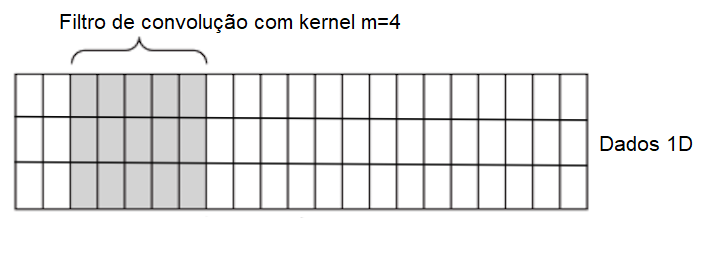
\includegraphics[width=0.9\textwidth]{figuras/fig_11.png}
   \fonte{\cite{Verma2020}}
\end{figure}

\begin{figure}[h]
  \centering
  \caption{Convolução em dados 3D.}
   \label{fig:cnn_convolution_3d}
   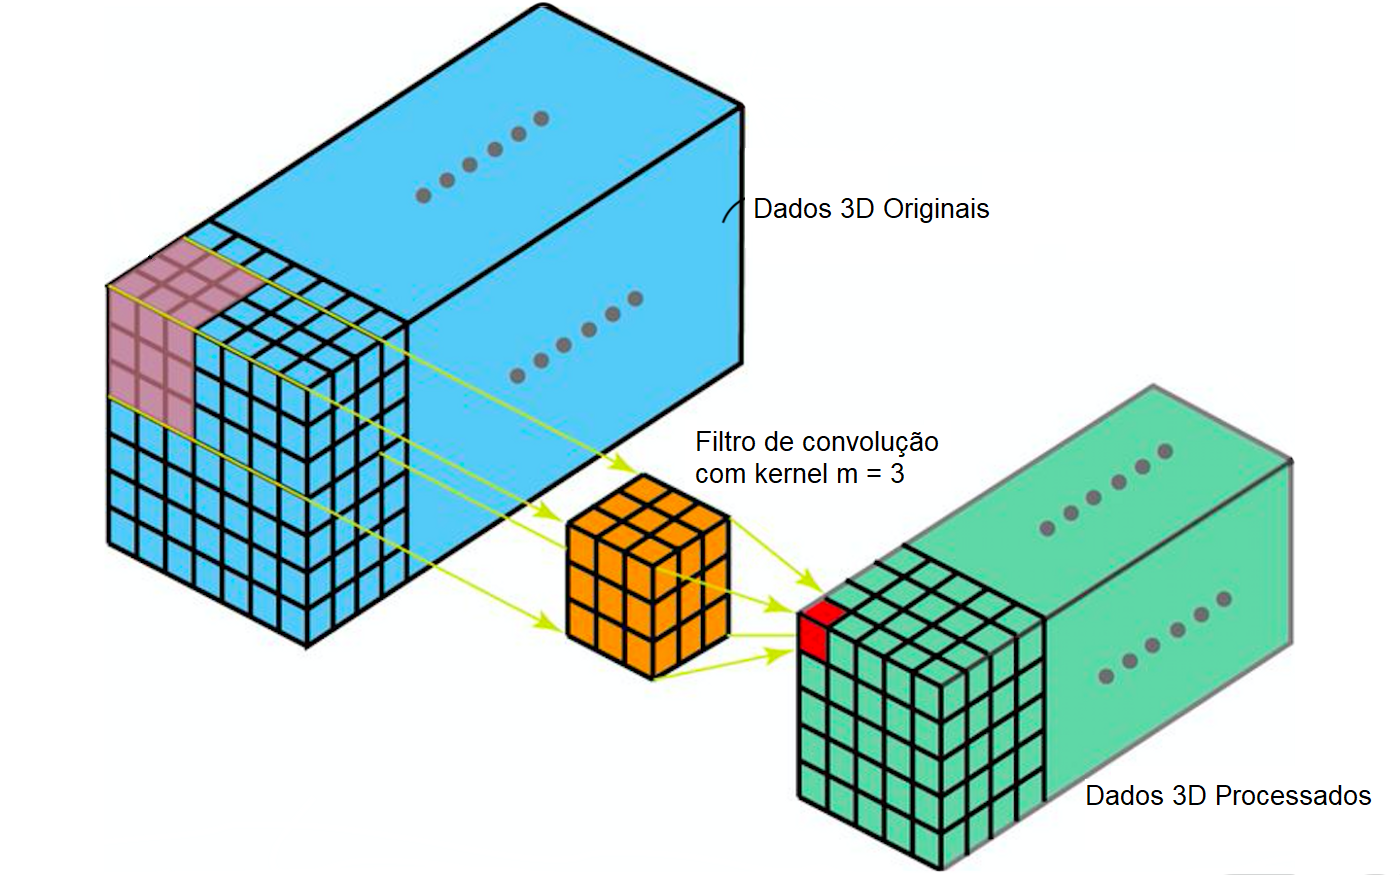
\includegraphics[width=0.8\textwidth]{figuras/fig_12.png}
   \fonte{\cite{Verma2020}}
\end{figure}

\subsection{Convolutional Long Short-Term Memory}

A ConvLSTM é um tipo de RNN variante da LSTM \cite{Salman2018}. Nestas redes existem operações de convolução dentro da célula de LSTM, de forma que as estruturas de convolução são aplicadas tanto na transição de entrada para estado, quanto nas transições de estado para estado. Desta forma, todas as operações de multiplicação de matrizes interna são substituídas por convoluções \cite{Rahman2019}. Neste ponto se mostra evidente a diferença para a híbrida CNN-LSTM, nas quais estruturas de convolução (CNN) são aplicadas como a primeira camada e sequencialmente na segunda camada é aplicada LSTM \cite{Rahman2019}.

\subsection{Convolutional Neural Network Long Short-Term Memory}

A CNN-LSTM constitui um tipo de rede neural híbrida que utiliza de ambas camadas de convolução (CNN) e recorrência (LSTM) \cite{Deep2019}. Nestas redes, os sinais são inicialmente agrupados em sequências temporais, e cada sequência é subdividida em blocos menores, as subsequencias. Nestas subsequências são aplicadas camadas de convolução para extração de características complexas \cite{Deep2019}. Em seguida, estas características são agrupadas novamente na sequência original e empregadas em camadas recorrentes, para interpretar a sequência temporal das características produzidas.

\section{Métricas de Avaliação}

Para mensurar os resultados dos experimentos foram adotadas métricas comumente utilizadas em problemas de classificação: acurácia, precisão, \textit{recall} e \textit{f1-score} \cite{Rodrigues2020,Rodrigues2021,Shung2020}. Em um problema de classificação, os resultados podem ser classificados em Verdadeiros Positivos (VP), sendo a classificação correta da classe Positivo; Verdadeiros Negativos (VN), a classificação correta da classe Negativo; Falsos Positivos (FP), erro em que o modelo previu a classe Positivo quando o valor real era classe Negativo; e Falsos Negativos (FN), erro em que o modelo previu a classe Negativo quando o valor real era classe Positivo \cite{Rodrigues2020}. A \autoref{fig:classificacao_positivo_negativo} ilustra os resultados possíveis.

\begin{figure}[h]
  \centering
  \caption{Matriz confusão de classificação.}
   \label{fig:classificacao_positivo_negativo}
   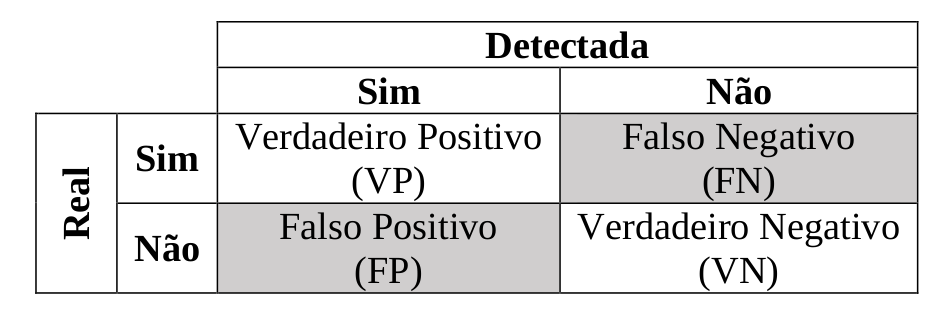
\includegraphics[width=0.6\textwidth]{figuras/fig_13.png}
   \fonte{\cite{Rodrigues2020}}
\end{figure}

A acurácia indica uma performance geral do modelo. Desta forma, consiste da proporção de amostras classificadas corretamente em relação ao total de amostras, considerando todas as classes de dados. A fórmula desta métrica é apresentada a seguir:

\begin{center}
  \[
  \textit{Acurácia} = \frac{VP + VN}{VP + VN + FP + FN}
  \]
\end{center}

Por outro lado, as métricas de precisão, \textit{recall} e \textit{f1-score} avaliam cada uma das classes de dados separadamente, de modo que se possa verificar problemas de desbalanceamento e viés. A precisão mede a proporção de amostras preditas corretamente em relação ao total de predições para determinada classe de dados, conforme a seguinte fórmula:

\begin{center}
  \[
  \textit{Precisão} = \frac{VP}{VP + FP}
  \]
\end{center}

A \textit{recall} mede a proporção de amostras preditas corretamente para determinada classe de dados em relação a todas as amostras reais daquela classe, conforme a seguinte fórmula:

\begin{center}
  \[
  \textit{Recall} = \frac{VP}{VP + FN}
  \]
\end{center}

Por fim, a \textit{f1-score} consiste da média harmônica de precisão e \textit{recall}, conforme a fórmula a seguir:

\begin{center}
  \[
  \textit{F1-Score} = \frac{2 * \textit{precisão} * \textit{recall}}{\textit{precisão} + \textit{recall}}
  \]
\end{center}

\chapter{Proposta}
\label{cap:proposta}

Nesta seção é detalhada a proposta de modelo adaptativo a ser desenvolvido de percepção veicular de ambiente e propriocepção veicular. Nas próximas seções é detalhada a metodologia e materiais adotados, andamento da pesquisa, resultados preliminares obtidos e cronograma de atividades.

\section{Metodologia}

Para o desenvolvimento deste trabalho, inicialmente foi realizado o levantamento do estado-da-arte sobre percepção veicular de ambiente e propriocepção veicular, através de sinais de sensores inerciais. Este levantamento se deu por intermédio de produção de uma Revisão Sistemática da Literatura (RSL), em bases de dados relevantes na área de computação. Através dessa sistemática, diversas lacunas de pesquisa foram identificadas conforme discorrido no capítulo \ref{cap:revisao}, com a delimitação de escopo desta pesquisa. Baseando-se nas lacunas de pesquisa, o desenvolvimento da metodologia de percepção adaptativa se dá em três etapas, sendo elas a coleta de dados, o pré-processamento e processamento. 

Na etapa de de coleta de dados, são utilizadas duas redes de sensores no veículo, sendo cada uma destas constituídas por um \textit{Single-Board Computer} (SBC) Raspberry Pi e três placas MPU-9250, cada uma equipada com um acelerômetro, um giroscópio e um magnetômetro. Também foi utilizado uma fonte externa de GPS, com produção de dados de localização e velocidade. Para definição dos referenciais, utilizou-se posicionamento controlado, uma vez que melhor se adéqua ao estudo. Sendo assim, o posicionamento das placas foi realizado de forma que os eixos do referencial do sensor coincidem com os do veículo, não sendo necessário mapear. As redes com as placas MPU-9250 foram distribuídas no veículo de forma a considerar os dados provindos de pontos com diferentes fatores de dependência, uma vez que a análise busca estabelecer qual ponto fornece os dados que produzem melhores resultados. Sendo assim, foram distribuídas no veículo da seguinte maneira: cada extremidade do eixo frontal (lado direito e esquerdo) recebeu uma das redes, onde anexou-se uma placa na bandeja da suspensão, localizando-se abaixo e próximo à suspensão veicular; outra placa acima e próxima à suspensão, anexada na lataria; e outra placa anexada na \textit{dashboard} do veículo, dentro da cabine. A taxa de amostragem não foi restringida, atingindo próximo a 1 kHz, uma vez que para os experimentos será realizado \textit{downsampling} para verificar a melhor taxa. Foi empregada a faixa de medição máxima (8g), uma vez que em testes exploratórios foi observado em algumas ocasiões a produção de valores de até aproximadamente 7.5g. 

Após, na etapa de pré-processamento se busca melhorar os dados brutos antes de serem parametrizados a técnica de reconhecimento de padrões. Sendo assim, será utilizada técnica empregada por \cite{Li2018} para aproximar as localizações e velocidade em uma taxa próxima a dos sensores inerciais. Desta forma, são produzidos dados mais próximos aos reais em cada amostra. Nesta etapa também será integrado o modelo matemático \textit{Quarter Car}, de forma que suas fórmulas condicionem os valores dos sensores inerciais ao veículo no qual os dados foram captados. Também será investigado se o emprego de formalismos matemáticos que descrevem as relações físicas entre as variáveis, como aceleração centrífuga a partir da aceleração, velocidade e curvatura, podem melhorar os resultados se aplicados como pré-processamento, ao invés de deixar a rede neural descobrir suas relações.

Na etapa de processamento serão aplicadas os dados pré-processados à uma técnica de \textit{Deep Learning}, sendo ela redes neurais recorrentes do tipo LSTM. Com o desenvolvimento das percepções, serão fornecidas as mesmas como mais uma das entradas para outras percepções, como forma de verificar melhorias dado sua correlação. A validação da adaptabilidade será feita com base nos \textit{datasets} produzidos na primeira etapa. Para isso, serão coletados ao menos quatro conjuntos de dados com diferenças de propriedades veiculares, de ambiente e de condução. Três dos \textit{datasets} serão utilizados parcialmente para treinamento e o restante para validação, sendo o quarto \textit{dataset} utilizados somente para validação, de forma a verificar o comportamento do modelo em um contexto desconhecido.

\section{Andamento da Proposta e Resultados Preliminares}

A pesquisa prática encontra-se em estágio inicial de desenvolvimento. Foi produzido para os testes preliminares um \textit{dataset} com os quais foram aplicados reconhecimento de algumas percepções. Este \textit{dataset} é composto de dados amostrados no seguinte contexto: um veículo trafegando em vias com três diferentes tipos de superfície, com a presença de eventos transientes como buracos, lombadas, curvas, etc., com variações no modo de condução, tal como diferentes velocidades. Utilizando-se deste \textit{dataset}, foram produzidas três percepções veiculares diferentes, a fim de demonstrar ser possível realizar este tipo de reconhecimento nos dados dos sensores, assim como validar que a técnica de \textit{Deep Learning} proposta é adequada ao problema de pesquisa. Os reconhecimentos realizados foram dois de percepção de ambiente, sendo um evento persistente de tipo de composição de superfície e outro transiente, sendo as lombadas; e um reconhecimento de propriocepção, o evento transiente de curvas.

Para realização dos testes, após a criação de diversos modelos de redes neurais profundas, chegou-se a rede detalhada na Figura \ref{fig:rede_proposta}. Esta rede é composta de uma camada de entrada, a qual recebe sequencias de 25 amostras (2,5 segundos) para formação da saída. São parametrizadas sete variáveis, sendo aceleração e rotação nos três eixos captados abaixo da suspensão veicular, e a velocidade. Posteriormente, estes dados passam para uma camada de convolução, a fim de filtrá-los e melhorá-los. Nesta etapa, estudos anteriores geralmente empregaram métodos estatísticos, tais como média móvel simples, para suavizar os dados e remover ruídos. Em seguida, os dados são parametrizados a duas camadas de LSTM, conhecidas como \textit{stacked} LSTM. Estas camadas são responsáveis por extrair as características dos dados. Alguns estudos anteriores empregaram nesta etapa métodos como o desvio padrão, para extração de característica de vibração dos sinais. Por fim, os dados são passados a camada de saída, resultando em uma ou mais classes, conforme a percepção produzida.

\begin{figure}[h!]
  \centering
  \caption{Rede Neural Profunda.}
   \label{fig:rede_proposta}
   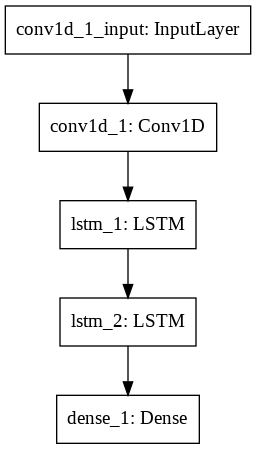
\includegraphics[width=0.3\textwidth]{figuras/fig4_2.png}
   \fonte{O autor.}
\end{figure}

O primeiro teste se concentrou no reconhecimento do tipo de superfície da vida. Foram reconhecidos três tipos diferentes, sendo pavimento rígido (asfalto), pavimento flexível (paralelepípedo ou hexagonal) e sem pavimentação (terra). A rede neural profunda para este reconhecimento obteve uma acurácia de 99\%, com um Erro Médio Quadrático (\textit{Mean Squared Error} - MSE) de 0.0000045885. O reconhecimento de pavimento asfáltico obteve o melhor resultado, com Erro Médio Absoluto (\textit{Mean Absolute Error} - MAE) de 0.000023. Em seguida, o reconhecimento de terra obteve MAE de 0.000054, e o reconhecimento de paralelepípedo/hexagonal obteve MAE de 0.000064. As Figuras \ref{fig:resultado_asfalto}, \ref{fig:resultado_paralelepipedo} e \ref{fig:resultado_terra} detalham os resultados.

O segundo teste foi voltado ao reconhecimento de lombadas. Sendo assim, envolveu lombadas tanto em pavimento asfáltico, quando em paralelepípedo, de diversas dimensões. A rede neural profunda para esse reconhecimento também obteve acurácia de 99\% e um MSE de 0.0005878024. O MAE foi de 0.000012, e os resultados são detalhados na Figura \ref{fig:resutlado_lombada}. Por fim, no terceiro teste foi realizado o reconhecimento de curvas à direita e à esquerda, sendo elas leves ou acentuadas. A rede obteve acurácia de 92\% com um MSE de 0.0020476580. Para curvas a esquerda, o MAE foi de 0.004028, e para a direita, de 0.010060. Os resultados são detalhados na Figura \ref{fig:resultado_curva_esquerda} e \ref{fig:resultado_curva_direita}.

De modo geral, é possível observar o bom desempenho a rede em filtrar sinais, extrair características e reconhecer os padrões, fazendo com que a LSTM seja interessante para este problema. Em relação à adaptabilidade, alguns fatores de dependência já foram agregados, como a velocidade e características sensoriais descritas na seção anterior. Sendo assim, faltam agregar os demais fatores ao modelo, e prosseguir com testes para outras percepções e outros contextos, com a produção de novos \textit{datasets}.

\begin{figure}[h!]
  \centering
  \caption{Reconhecimento de Pavimento Rígido (Asfalto).}
   \label{fig:resultado_asfalto}
   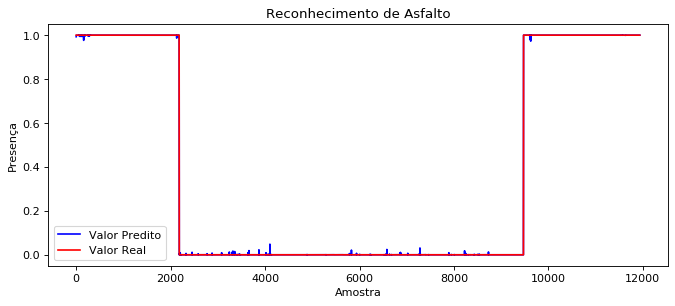
\includegraphics[width=1\textwidth]{figuras/fig4_2_1.png}
   \fonte{O autor.}
\end{figure}

\begin{figure}[h!]
  \centering
  \caption{Reconhecimento de Pavimento Flexível (Hexagonal ou Paralelepípedo).}
   \label{fig:resultado_paralelepipedo}
   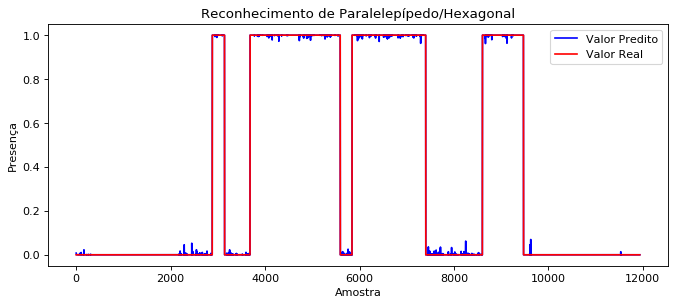
\includegraphics[width=1\textwidth]{figuras/fig4_2_2.png}
   \fonte{O autor.}
\end{figure}

\begin{figure}[h!]
  \centering
  \caption{Reconhecimento de Sem Pavimento (Terra).}
   \label{fig:resultado_terra}
   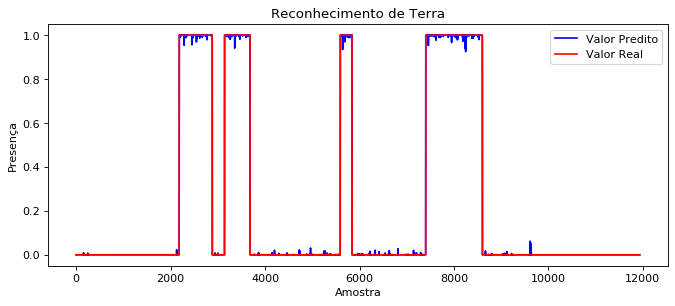
\includegraphics[width=1\textwidth]{figuras/fig4_2_3.png}
   \fonte{O autor.}
\end{figure}

\begin{figure}[h!]
  \centering
  \caption{Reconhecimento de Lombada.}
   \label{fig:resutlado_lombada}
   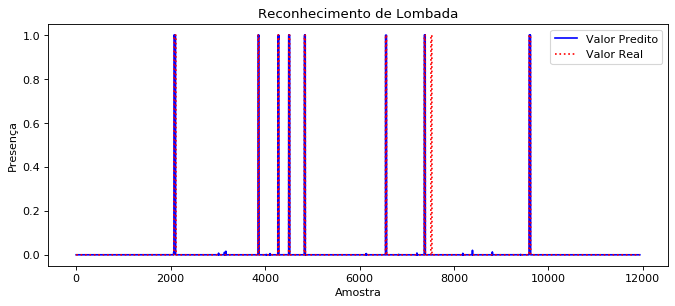
\includegraphics[width=1\textwidth]{figuras/fig4_2_4.png}
   \fonte{O autor.}
\end{figure}

\begin{figure}[h!]
  \centering
  \caption{Reconhecimento de Curva à Esquerda.}
   \label{fig:resultado_curva_esquerda}
   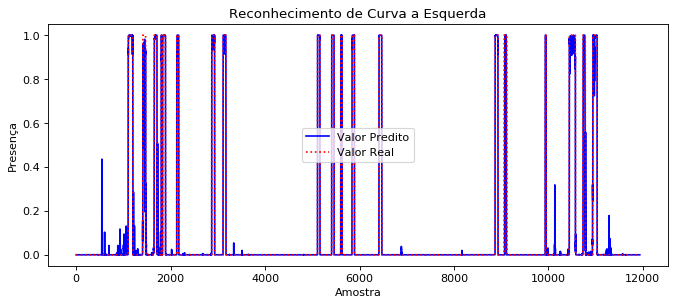
\includegraphics[width=1\textwidth]{figuras/fig4_2_5.png}
   \fonte{O autor.}
\end{figure}

\begin{figure}[h!]
  \centering
  \caption{Reconhecimento de Curva à Direita.}
   \label{fig:resultado_curva_direita}
   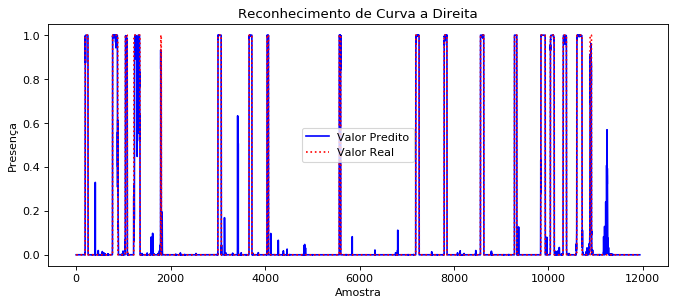
\includegraphics[width=1\textwidth]{figuras/fig4_2_6.png}
   \fonte{O autor.}
\end{figure}

\clearpage 
\section{Cronograma}

Abaixo é apresentado o cronograma a ser seguido com o intuito de cumprir as etapas da pesquisa e os requisitos que regulamentam o curso.

\begin{figure}[h!]
  \centering
  \caption{Cronograma de atividades.}
   \label{fig:proprioception_occurrence}
   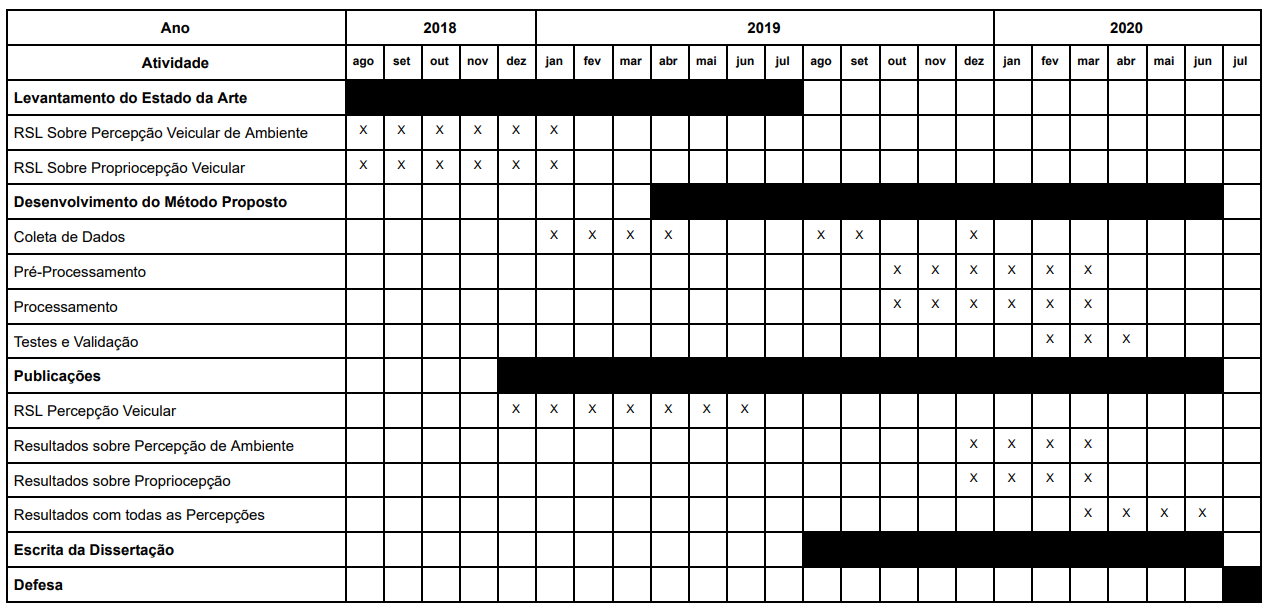
\includegraphics[width=1\textwidth]{figuras/fig4.png}
   \fonte{O autor.}
\end{figure}



%%%%%%%%%%%%%%%%%%%%%%%%%%%%%%%%%%%%%%%%%%%%%%%%%%%%%%%%%%%%%%%%%%%%
%%% Elementos pós-textuais                                       %%%
%%%%%%%%%%%%%%%%%%%%%%%%%%%%%%%%%%%%%%%%%%%%%%%%%%%%%%%%%%%%%%%%%%%%

\postextual
\bibliography{bibliografia}

\end{document}
